\chapter{统计学}
统计学萌芽于欧洲,16世纪伽利略Galileo Galilei为解答赌徒们的问题,提出了概率论的基本原理。17世纪中叶,帕斯卡Blaise Pascal
\footnote{布莱斯·帕斯卡Blaise Pascal(1623 $\sim$ 1662)是法国物理学家、哲学家和神学家,还是一位伟大的数学家和统计学家,他唯一留给世人的是载录其理论思想的《思想录》,虽未形成系统的理论框架,仍然具有重要的参考价值。他曾经提出了一个著名的赌注,深刻影响了概率论、决策论的诞生,并促进存在主义、实用主义、唯意志论发展,后人称之为“帕斯卡的赌注”(Pascal's Wager):上帝要么存在,要么不存在。如果你相信上帝的存在,那么最坏的可能就是上帝本不存在,则在死后进入虚无世界,你没有任何损失;若上帝确实存在,那么你将获得永生。如果你拒绝信仰,则最好的结果就是虚无,但最坏的结果就是承受永世的地狱之苦。一个理性的人,就应该相信上帝的存在。}
和费马Pierre de Fermat关于“得点问题”的讨论,奠定了\textbf{概率论}(Probability Theory)的基础。17世纪末18世纪初统计学开始蓬勃发展。19世纪末,由于英国探险家、人类学家和优生学家法兰西斯·高尔顿Francis Galton和统计学家卡尔·皮尔逊Karl Pearson的突出贡献,\textbf{描述统计学}(Descriptive Statistics)正式诞生。\textbf{推论统计学}
(Inferential Statistics)是研究如何根据样本数据去推断总体统计特征,先驱人物是英国统计学家威廉·格赛特William Sealy Gosset和罗纳德·费舍尔Ronald Aylmer Fisher。最初将统计学应用于教育与心理方面研究的是高尔顿,而对教育统计做出重要贡献的是心理学家查尔斯·爱德华·斯皮尔曼Charles Edward Spearman。

\ornamento

\section{概率论基础}
概率论与数理统计(Probability and Mathematical Statistics)研究的对象是随机现象。
在一定的条件下,并不总是出现相同结果的现象称为\textbf{随机现象}。随机现象的结果不止一个,并且人们事先并不知道哪个结果出现。如果只有一个结果,那么该现象称为\textbf{确定性现象}。在相同条件下可以重复的随机现象又称作
\textbf{随机试验}(Random Trial),比如抛硬币、掷骰子的试验等。自然界中还有很多无法重复的随机现象,比如某场球赛的输赢、某个时段的经济增长速度等。

随机现象的一切可能的基本结果组成的集合称作\textbf{样本空间}(Sample Space),记作$\Omega=\{\omega\}$,其中$\omega$表示基本结果,又称为样本点,也是抽样时的基本单元。样本空间至少有两个样本点,只含有两个样本点的样本空间是最简单的样本空间。如果样本点的数目有限或可数,则称该样本空间为离散样本空间;如果样本点的数目不可数,则称该样本空间是连续样本空间。

随机现象的某些样本点组成的集合称作\textbf{随机事件},简称\textbf{事件}。样本空间$\Omega$的最大子集(即$\Omega$自身)称作\textbf{必然事件}、最小子集(即空集$\emptyset$)称作\textbf{不可能事件}。用来表示随机现象结果的变量称作\textbf{随机变量}。

\begin{example}
骰子(亦作色子)是一种古老的赌具,多为正立方体六面骰,各面刻有一至六个点数,并且彼此相对的两面数字之和为七。骰子最早出现在两千年前的埃及,古埃及人称其“astragal”。在中国,相传骰子是由三国时的文学家曹植所发明,最初用作占卜工具,后来演变成后宫嫔妃的游戏,根据掷骰子的点数赌酒或赌丝绸香袋等物。当时骰子的点穴上涂的是黑色,唐代时增加描红。

赌场内的荷官摇掷骰子透过骰子的点数定输赢,每一场赌局投掷骰子的点数都可能不同。荷官投掷骰子的事件可以看作是一个随机事件,记作$X$,所有可能的投掷结果构成样本空间$\Omega=\{1,2,3,4,5,6\}$,“投掷的骰子点数大于4”的事件可以使用“$X>4$”表示。
\end{example}

随机事件的不同结果的发生存在不同程度的可能性,有些结果可能性大有些可能性小。概率论最基本的一个问题是定义随机事件的概率,以刻画事件发生的可能性。16世纪,意大利学者Gerolamo Cardano
\footnote{Gerolamo Cardano(1501--1576),意大利数学家、医学家、物理学家,统计学创始人。1526年获帕维亚大学医学博士学位,后成为欧洲名医,曾任英国国王爱德华六世的御医,并曾任教于帕维亚大学、博洛尼亚大学。他学识渊博,一生写作出版各类文章、书籍200多种,被誉为百科全书式的学者。
他的家庭生活非常不幸。他最喜爱的大儿子詹巴蒂斯塔因杀死不忠的妻子于1560年被判死刑。他的女儿沦为妓女,死于梅毒。他的另一个儿子是个赌徒,经常偷窃他的财物。他自己因为推算耶稣的出生星位,被指控为大逆不道,于1570年入狱,并失去教职。更为可悲的是,他的儿子参与了指控。出狱后他移居罗马,获得了教皇格里高利十三世(Pope Gregory XIII)的年金资助,完成了自己的自传。据说,他七十一岁时通过占星术推算出自己将在1576 年9月21 日去世,但是到那一天时,他活得像头壮牛;为了保全自己大星象学家的名声,他自杀了。}
开始研究赌博游戏中的一些简单问题,其死后发表的《论赌博游戏》(\textit{Liber de ludo aleae})给出了一些概率论的基本概念和定理,被认为是第一部概率论著作。在Cardano以后约三百年的时间里,Blaise Pascal、Pierre de Fermat、Jacob Bernoulli等数学家都在古典概率计算、公式推导和扩大应用等方面做了重要的工作。1812年,法国数学家Pierre-Simon Laplace在《概率的分析理论》(\textit{Th\'{e}orie analytique des probabilit\'{e}s})中给出概率的古典定义:事件$A$的概率等于一次试验中出现事件$A$的可能结果数目与该事件中所有可能结果数目之比。古典定义通过简单明了的方式定义了事件的概率,并给出简单可行的方法。古典定义是在经验事实的基础上,对被考察事件的可能性进行逻辑分析后得到的事件概率。古典定义的基本假设有两个:(甲)随机事件可能结果总数有限;(乙)每个结果的出现有同等可能。Jacob Bernoulli在研究古典概率时发现Bernoulli大数定律,即“频率具有稳定性”,从而可以“用频率估计概率”。

概率论发展的历史,诞生过概率的古典定义、概率的几何定义、概率的频率定义和概率的主观定义。1900年,38岁的德国数学家David Hilbert在世界数学家大会上提出建立概率公理系统的问题,也就是著名的Hilbert 23个问题中的第6个问题。20世纪初完成的勒贝格测度与积分理论,以及随后发展的抽象测度和积分理论,为概率论公理体系的建立奠定了基础。1933年,前苏联数学家Andrey Kolmogorov\cite{Kolmogorov1951Foundations}运用集合论和测度论正式给出概率严密的公理化定义,既概括了古典定义、统计定义的基本特性,又避免了各自的局限。概率论公理体系的出现是概率论发展史上的一个里程碑,至此概率论才真正成为严格的一个数学分支。

\begin{definition}[$\sigma$-代数与可测空间]
假设$\Omega$是一个样本空间,$\mathscr F$是$\Omega$的某些子集所构成的集合类(Collection)。如果$\mathscr F$满足:
\begin{itemize}
  \item $\Omega\in \mathscr F$;
  \item \textbf{余集封闭}:如果$A\in \mathscr F$,则$\bar A=\Omega\setminus A\in \mathscr F$;
  \item \textbf{可列并封闭}:如果$A_n\in \mathscr F$,$n=1,2,\ldots$,则$\bigcup\limits_{n=1}^{\infty}A_n\in \mathscr F$。
\end{itemize}
则称$\mathscr F$为\textbf{$\sigma$-代数}(Sigma-Algebra)、\textbf{Borel域}(Borel Field)或\textbf{事件域}(Field of Events),$(\Omega,\mathscr F)$称作\textbf{可测空间}(Measurable Space)。
\end{definition}
根据定义可以推知:
\begin{itemize}
  \item $\emptyset\in \mathscr F$;
  \item \textbf{差集封闭}:如果$A,B\in \mathscr F$,则$A\setminus B\in \mathscr F$;
  \item \textbf{有限交、有限并、可列交封闭}:如果$A_n\in \mathscr F$,$n=1,2,\ldots$,则$\bigcap\limits_{i=1}^n A_n, \bigcup\limits_{i=1}^n A_n, \bigcap\limits_{n=1}^{\infty}A_n\in \mathscr F$。
\end{itemize}

\begin{definition}[概率与概率空间]
假设$(\Omega,\mathscr F)$是可测空间,$P(\cdot)$是定义在$\mathscr F$上的实值函数,如果满足:
\begin{itemize}
  \item \textbf{非负性公理}:对任意的$A\in \mathscr F$,都有$0\le P(A)\le 1$;
  \item \textbf{正则性公理}:$P(\Omega)=1$;
  \item \textbf{可列可加性公理}:对于两两互不相容事件$A_1,A_2,\ldots$($A_i\cap A_j = \emptyset$,$i\ne j$)有:
  \[
    P(\bigcup\limits_{i=1}^\infty A_i) = \sum\limits_{i=1}^\infty P(A_i),
  \]
\end{itemize}
则称$P(\cdot)$是可测空间$(\Omega,\mathscr F)$上的\textbf{概率}(Probability),$P(A)$为事件$A$的概率,$(\Omega,\mathscr F, P)$称作\textbf{概率空间}
(Probability Space)。
\end{definition}
根据定义可以推知:
\begin{itemize}
  \item \textbf{可减性}:如果$A,B\in \mathscr F$且$A\subset B$,则$P(B\setminus A) = P(B) - P(A)$;
\end{itemize}
如果事件列$\{A_n, n\ge 1\}$满足$A_n\subset A_{n+1}$,则称作单调增列,有$\lim\limits_{n\rightarrow \infty} A_n = \bigcup\limits_{i=1}^{\infty} A_i$;
如果事件列$\{A_n, n\ge 1\}$满足$A_n\supset A_{n+1}$,则称作单减增列,有$\lim\limits_{n\rightarrow \infty} A_n = \bigcap\limits_{i=1}^{\infty} A_i$。
\begin{itemize}
  \item \textbf{概率连续性}:如果事件列$\{A_n, n\ge 1\}$是单调减列或单调增列,则
  \[
    \lim_{n\rightarrow \infty} P(A_n) = P(\lim_{n\rightarrow \infty} A_n).
  \]
\end{itemize}

概率的解释与定义在争议中不断向前发展,从
概率的公理化定义刻画了概率的本质,但是没有明确指出具体地确定概率的方法。在公理化定义之前的概率的频率定义、古典定义、几何定义和主观定义都在一定场合下,存在各自确定概率的方法。在公理化定义范畴下,一一对应确定概率的频率方法、古典方法、几何方法和主观方法。

\begin{definition}[条件概率]
假设$(\Omega,\mathscr F, P)$是概率空间,$B\in \mathscr F$,且$P(B)>0$,如果对任意的$A\in \mathscr F$,记
\[
    P(A|B) = \frac{P(AB)}{P(B)},
\]
则称$P(A|B)$为事件$B$发生的条件下,事件$A$发生的\textbf{条件概率}(Conditional Probability)。
\end{definition}
由条件概率的定义可知:
\begin{itemize}
  \item \textbf{乘法公式}:设$A,B\in \mathscr F$,则有$P(AB)=P(A|B)P(B)$。一般地,如果$A_i\in \mathscr F, i=1,2,\ldots,n$,且$P(A_1 A_2\cdots A_n)>0$,则有\[P(A_1 A_2\cdots A_n)=P(A_1)P(A_2|A_1)P(A_3|A_1A_2)\cdots P(A_n|A_1A_2\cdots A_{n-1}).\]
  \item \textbf{全概率公式}:设$(\Omega,\mathscr F, P)$是概率空间,$A\in \mathscr F$,$B_i\in \mathscr F$,$i = 1,2,\ldots,n$,$B_i\cap B_j=\emptyset (i\ne j)$,且$\bigcup\limits_{i=1}^n B_i = \Omega$,$P(B_i)>0$,则有
      \[
        P(A) = \sum\limits_{i=1}^n P(A|B_i) P(B_i).
      \]
  \item \textbf{贝叶斯定理\footnote{Thomas Bayes(1701--1761),英国数学家,生前是一位受人尊敬的英格兰长老会牧师。他是一位自学成才的数学家,1742 年入选英国皇家学会会员,1763年在一篇论文中首次提到贝叶斯定理。为了证明上帝的存在,他发展了一套成熟的概率方法论。他的思想和方法对概率统计的发展产生了深远的影响,至今在许多领域都还有广泛应用。}}:设$(\Omega,\mathscr F, P)$ 是概率空间,$A\in \mathscr F$,$B_i\in \mathscr F$,$i = 1,2,\ldots,n$,$B_i\cap B_j=\emptyset (i\ne j)$,且$\bigcup\limits_{i=1}^n B_i = \Omega$,$P(B_i)>0$,$P(A)>0$,则有
      \[
        P(B_i|A) = \frac{P(B_i)P(A|B_i)}{\sum\limits_{i=1}^n P(A|B_i) P(B_i)}.
      \]
      一般地,若对任意的$A_1,\ldots,A_n\in \mathscr F$,都有$P(\bigcap\limits_{i=1}^n A_i) =\prod\limits_{i=1}^n P(A_i)$,则称$\mathscr F$是独立事件簇。
\end{itemize}

\begin{definition}[随机变量及其分布函数]
假设$(\Omega,\mathscr F, P)$是概率空间,$X=X(\omega)$是定义在$\Omega$上的实值函数。如果对任意的$x\in \mathbb R$,都有$X^{-1}((-\infty,x])=\{\omega: X(\omega)\le x\}\in \mathscr F$,则称$X(\omega)$是$\mathscr F$上的\textbf{随机变量}(Random Variable),简记作$X$。$F(x) = P(X\le x)=P(\{\omega: X(\omega)\le x\})=P(X^{-1}((-\infty,x]))$称作随机变量$X$的\textbf{累积分布函数}(Cumulative Distribution Function, CDF),简称\textbf{分布函数}。
\end{definition}
根据随机变量的分布函数的定义,我们可以得到下面几条性质:
\begin{itemize}
  \item $F(x)$是增函数:当$x_1<x_2$时有$F(x_1)\le F(x_2)$;
  \item $F(-\infty) = \lim\limits_{x\rightarrow -\infty} F(x)=0$,$F(+\infty) = \lim\limits_{x\rightarrow +\infty} F(x)=1$;
  \item $F(x)$右连续。
\end{itemize}
随机变量有两种类型:离散型和连续型随机变量。离散型随机变量的概率分布可以使用\textbf{概率分布列}或曰\textbf{概率质量函数}(Probability Mass Function, PMF)表示:$p_k = P(X=x_k),k=1,2,\ldots$,其分布函数为$F(x)=\sum\limits_{x\le x_k} p_k$;连续型随机变量的概率分布用\textbf{概率密度函数}(Probability Density Function, PDF)$f(x)$来描述,其分布函数$F(x)=\int_{-\infty}^x f(t)dt$。

\begin{definition}[多维随机变量及其分布函数]
假设$(\Omega,\mathscr F, P)$是概率空间,$X_i=X_i(\omega), i=1,2,\ldots,n$都是定义在$\Omega$上的实值函数。如果对任意的$x_i\in \mathbb R$,都有$X_i^{-1}((-\infty,x_i])=\{\omega: X_i(\omega)\le x_i\}\in \mathscr F$,则称$X(\omega)=(X_1(\omega),X_2(\omega),\ldots,X_n(\omega))$是\textbf{$n$维随机变量}或\textbf{随机向量},简记作$X=(X_1,X_2,\ldots,X_n)$。$F(x_1,x_2,\ldots,x_n) = P(X_1\le x_1,X_2\le x_2,\ldots, X_n\le x_n)$称作随机变量$X$的
\textbf{联合分布函数}(Joint Cumulative Distribution Function,JCDF)。
\end{definition}

对于二维随机变量$(X,Y)$,其联合分布函数$F(x,y)=P(X\le x, Y\le y)$是事件$\{X\le x\}$与事件$\{Y\le y\}$同时发生的概率。
\begin{definition}[二维离散随机变量与联合分布列]
如果二维随机变量$(X,Y)$只取有限个或可数的$(x_i,y_i)$,则称$(X,Y)$为二维离散随机变量,称
\[
    p_{ij} = P(X=x_i, Y=y_i),~~~i,j=1,2,\ldots
\]
为$(X,Y)$的\textbf{联合分布列}(Joint Probability Mass Function, JPMF)。
\end{definition}
\begin{definition}[二维连续随机变量与联合密度函数]
如果存在二元非负函数$p(x,y)$,使得二维随机变量$(X,Y)$的分布函数$F(x,y)$可表示为
\[
    F(x,y)=\int_{-\infty}^x \int_{-\infty}^y f(u,v) dv du,
\]
则称$(X,Y)$为二维随机变量,称$f(u,v)$为$(X,Y)$的\textbf{联合密度函数}(Joint Probability Density Function, JPDF)。
\end{definition}

\begin{definition}[边际概率分布函数]
如果在二维随机变量$(X,Y)$的联合分布函数$F(x,y)$中取$y\rightarrow +\infty$,由于$\{Y<+\infty\}$是必然事件,则称
\[
    \lim\limits_{y\rightarrow +\infty} F(x,y) = P(X\le x, Y\le +\infty) = P(X\le x),
\]
是$X$的\textbf{边际概率分布函数}(Marginal Distribution Function),记为
\[
    F_X(x) = F(x,+\infty).
\]
类似地,$F_Y(y)=F(+\infty,y)$称作$Y$的边际概率分布函数。
\end{definition}

在二维离散随机变量$(X,Y)$的联合分布列$\{P(X=x_i,Y=y_j)\}$中,对$j$求和所得的分布列
\[
    \sum\limits_{j=1}^\infty P(X=x_i,Y=y_j)=P(X=x_i),~~~i=1,2,\ldots
\]
称作$X$的边际概率分布列。类似地,对$i$求和所得的分布列
\[
    \sum\limits_{i=1}^\infty P(X=x_i,Y=y_j)=P(Y=y_j),~~~j=1,2,\ldots
\]
称作$Y$的边际概率分布列。

如果二维连续随机变量$(X,Y)$的联合概率密度函数为$f(x,y)$,由于
\begin{eqnarray}
  \nonumber F_X(x) = F(x,+\infty) =\int_{-\infty}^x \Bigg(\int_{-\infty}^{+\infty} f(u,v)dv\Bigg) du \triangleq \int_{-\infty}^x f_X(u)du,\\
  \nonumber F_Y(y) = F(+\infty,y) =\int_{-\infty}^y \Bigg(\int_{-\infty}^{+\infty} f(u,v)du\Bigg) dv\triangleq \int_{-\infty}^y f_Y(v)dv,
\end{eqnarray}
其中$f_X(x)$和$f_Y(y)$分别称作$X$的边际概率密度函数、$Y$的边际概率密度函数(Marginal Density Function)。

\section{随机变量的数字特征}%Numerical Characteristics
\begin{definition}[数学期望]
假设$X$是定义在概率空间$(\Omega,\mathscr F, P)$上的随机变量,如果$\int_{\Omega} |X| dP <\infty$,就称$X$的\textbf{数学期望}(Expectation)或均值存在,或称$X$是可积的,记作$E(X)$,并有下列定义:
\[
    E(X) = \int_{\Omega} X dP.
\]
如果$X$是离散型随机变量,如果级数$\sum\limits_{i=1}^{+\infty} |x_i| p_i$收敛,则$E(X)=\sum\limits_{i=1}^{+\infty} x_i p_i$是随机变量$X$的数学期望。如果$X$是连续型随机变量,如果积分$\int_{-\infty}^{+\infty} |x| f(x)dx$收敛,则$E(X)=\int_{-\infty}^{+\infty} x f(x)dx$是随机变量$X$的数学期望。
\end{definition}

\begin{definition}[条件分布]
对一切使$f_Y(y)>0$的$y$,给定$Y=y$条件下$X$的条件分布函数(Conditional Distribution Function)和条件密度函数(Conditional Density Function)分别为
\begin{eqnarray}
  F(x|y) &=& \int_{-\infty}^x \frac{f(u,y)}{f_Y(y)} du,\\
  f(x|y) &=& \frac{f(x,y)}{f_Y(y)} = \frac{f_X(x) f(y|x)}{\int_{-\infty}^{+\infty} f_X(x) f(y|x) dx}.
\end{eqnarray}
\end{definition}

\begin{definition}[条件数学期望]
设$X$和$Y$是随机变量,对一切使$f_Y(y)>0$的$y$,给定$Y=y$条件下$X$的期望定义如下:
\[
    E(X|Y=y) = \int_{-\infty}^{+\infty} xf(x|y)dx.
\]
%http://www.cnblogs.com/murongxixi/p/3477962.html
%http://www.jdl.ac.cn/user/lyqing/StatLearning/Statistical09Fall.html
\end{definition}
条件期望$E(X|Y=y)$是$y$的函数,对$y$的不同取值,条件期望$E(X|Y=y)$的取值也在变化。为此,我们记$g(y) = E(X|Y=y)$。我们还可以将条件期望看做是随机变量$Y$的函数,记作$E(X|Y)=g(Y)$。

\begin{theorem}[重期望公式]
设$(X,Y)$是二维随机变量,且$E(X)$存在,则$E(X)=E(E(X|Y))$。
\end{theorem}
\begin{proof}
假设$(X,Y)$的联合密度函数是$f(x,y)$,由$f(x,y)=f(x|y)f_Y(y)$可得:
\[
\begin{array}{lcl}
    E(X) & = & \int_{-\infty}^{+\infty} \int_{-\infty}^{+\infty} x f(x,y) dx dy\\
    &=& \int_{-\infty}^{+\infty}\big(\int_{-\infty}^{+\infty} xf(x|y) dx\big) f_Y(y) dy\\
    &=& \int_{-\infty}^{+\infty} E(X|Y=y) f_Y(y) dy\\
    &=& \int_{-\infty}^{+\infty} g(y) f_Y(y) dy\\
    &=& E(g(Y)) = E(E(X|Y)).
\end{array}
\]
证毕。
\end{proof}
我们下面来看条件期望的一些基本性质:
\begin{property}[独立性]
如果$X$和$Y$是两个独立随机变量,则对于任意使$f_Y(y)>0$的$y$都有\[E(X|Y=y)=E(X).\]
\end{property}
\begin{proof}
由$X$和$Y$的独立性可知$f(x,y)=f_X(x) f_Y(y)$,则$f(x|y)=\frac{f(x,y)}{f_Y(y)} = f_X(x)$,按照条件期望的定义则有
\[
    E(X|Y=y) = \int_{-\infty}^{+\infty} xf(x|y) dx = \int_{-\infty}^{+\infty} x f_X(x) = E(X).
\]
证毕。
\end{proof}
\begin{property}
设$h$是一个实值函数,对于任意使$f_Y(y)>0$的$y$都有$E(h(Y)|Y)=h(Y)$。
\end{property}
\begin{proof}
对于任意的$y\in \mathbb R$,如果给定$y$,则条件概率$f(h(Y) = h(y) | Y=y)=1$。根据定义可知
\[
\begin{array}{lcl}
    E(h(Y)|Y=y) = h(y) f(h(Y) = h(y) | Y=y) = h(y),
\end{array}
\]
那么$E(h(Y)|Y)=h(Y)$。
\end{proof}

\begin{property}[线性相加性]
设$X_1$、$X_2$和$Y$都是随机变量,$\alpha_1,\alpha_2\in \mathbb R$,则
\[
    E(\alpha_1 X_1 + \alpha_2 X_2|Y=y)=\alpha_1 E(X_1|Y=y) + \alpha_2 E(X_2|Y=y).
\]
\end{property}
\begin{proof}
我们直接按照条件期望的定义推导:
\[
    \begin{array}{lcl}
        E(\alpha_1 X_1 + \alpha_2 X_2|Y=y) &=& \int_{-\infty}^{+\infty} \int_{-\infty}^{+\infty} \alpha_1 u + \alpha_2 v f(X_1=u, X_2=v|Y=y) dudv\\
        &=&\alpha_1 \int_{-\infty}^{+\infty} \int_{-\infty}^{+\infty} u f(X_1=u, X_2=v|Y=y) dudv + \\
        &&\alpha_2 \int_{-\infty}^{+\infty} \int_{-\infty}^{+\infty} v f(X_1=u, X_2=v|Y=y) dudv\\
        &=& \alpha_1 \int_{-\infty}^{+\infty}  u f(X_1=u|Y=y) du + \alpha_2 \int_{-\infty}^{+\infty}  v f(X_2=v|Y=y) dv\\
        &=& \alpha_1 E(X_1|Y=y) + \alpha_2 E(X_2|Y=y).
    \end{array}
\]
证毕。
\end{proof}

\begin{property}
设$X$和$Y$是随机变量,$g$和$h$是实值函数,则$E[g(X)h(Y)] = E[h(Y)E(g(X)|Y)]$。
\end{property}
\begin{proof}
根据条件期望的定义可以推导:
\[
    \begin{array}{lcl}
        E[g(X)h(Y)] &=& \int_{-\infty}^{+\infty} \int_{-\infty}^{+\infty} g(x) h(y) f(x,y) dxdy\\
        &=& \int_{-\infty}^{+\infty} h(y) f_Y(y) (\int_{-\infty}^{+\infty} g(x) f(x|Y=y) dx) dy\\
        &=& \int_{-\infty}^{+\infty} h(y) E(g(X)|Y=y) f_Y(y) dy\\
        &=& E[h(Y)E(g(X)|Y)].
    \end{array}
\]
证毕。
\end{proof}

\begin{definition}[原点矩和中心矩]
假设$g(x)$是$\mathbb R$上的Borel可测函数,若其数学期望存在$E(|g(x)|) < \infty$,则有
\[
    E(g(X)) = \int_\Omega g(X) dP = \int_{-\infty}^{+\infty} g(x) f(x) dx.
\]
如果$g(X)=X^k, k\in \mathbb N$的数学期望存在,就称
\[
    E(X^k) = \int_{-\infty}^{+\infty} x^k f(x) dx
\]
为$X$的\textbf{$K$阶原点矩}(K-th Moment about the Origin)。如果$g(X)=|X|^k, k\in \mathbb N$的数学期望存在,称
\[
    E(|X|^k) = \int_{-\infty}^{+\infty} |x|^k f(x) dx
\]
为$X$的\textbf{$K$阶绝对原点矩}(K-th Absolute Moment about the Origin)。如果$g(X)=(X-E(X))^k, k\in \mathbb N$的数学期望存在,称
\[
    E((X-E(X))^k) = \int_{-\infty}^{+\infty} (x-E(X))^k f(x) dx
\]
为$X$的\textbf{$K$阶中心矩}(K-th Central Moment)。如果$g(X)=|X-E(X)|^k, k\in \mathbb N$的数学期望存在,称
\[
    E(|X-E(X)|^k) = \int_{-\infty}^{+\infty} |x-E(X)|^k f(x) dx
\]
为$X$的\textbf{$K$阶绝对中心矩}(K-th Absolute Central Moment)。
\end{definition}

\begin{definition}[方差]
我们称随机变量$X$的\textbf{二阶中心矩}为\textbf{方差}(Variance),记作$\var(X)$,则有
\[
    \var(X) = E((X-E(X))^2) = \int_{-\infty}^{+\infty} (x-E(X))^2 f(x) dx =  E(X^2) - (E(X))^2.
\]
\end{definition}

\begin{theorem}
对于随机变量$X$,如果对任意的$k\in \mathbb N$都有$E(|X|^k)<\infty$,则对所有的正整数$i<k$都有$E(|X|^i)<\infty$。
\end{theorem}
\begin{proof}
假设随机变量$X$是连续的,并且其概率密度函数是$f(x)$,则对于$i<k$有
\[
\begin{array}{lcl}
    E(|X|^i) &=& \int_{-\infty}^{+\infty} |x|^i f(x) dx\\
    &=& \int_{|x|\le 1} |x|^i f(x) dx + \int_{|x|> 1} |x|^i f(x) dx\\
    &\le& \int_{|x|\le 1} f(x) dx + \int_{|x|> 1} |x|^k f(x) dx\\
    &\le& P(|X|\le 1) + E(|X|^k),
\end{array}
\]
根据假设$E(|X|^k)<\infty$,必然有$E(|X|^i) < \infty$。
\end{proof}
由此可知,只要$E(X^2)<\infty$,则变量$X$的期望和方差都存在。

如果我们知道随机变量的分布函数,就可以很容易地计算出随机变量的各种数值特征,如均值、方差和其他各高阶矩。通常,计算随机变量的各阶矩,往往要进行求和或积分运算。实际上,我们可以简化随机变量各阶矩的积分或加和运算,并建立起各阶矩的统一形式。我们下面介绍两个重要的分析工具:\textbf{矩母函数}(Moment Generating Function)与\textbf{特征函数}(Characteristic Function),它们可以把独立随机变量和分布的卷积运算转换为乘法运算,将随机变量各阶原点矩的计算转换成简单的微分计算,甚至可以将随机变量序列的极限分布转换成一般函数极限问题。

\begin{definition}[矩母函数]
设$X$是一个随机变量,函数
\[
    \psi(t) = E(e^{tX}) = \int_{-\infty}^{+\infty} e^{tx} f(x)dx, -\infty < t < \infty,
\]
称作$X$的\textbf{矩母函数}(Moment Generating Function, MGF)。
\end{definition}
矩母函数$\psi(t)$对应随机变量$X$密度函数$f(x)$的\textbf{拉普拉斯变换}(Laplace Transformation),它只与随机变量$X$的分布函数有关,如果随机变量$X$与$Y$ 的分布函数相同,则它们的矩母函数也相同。如果随机变量$X$有界(Bounded),则矩母函数$\psi(t)$对所有的$t$都是有限的(Finite)。否则,矩母函数$\psi(t)$ 可能对于某些$t$有限,而对其他$t$却不是有限的。唯一可以确定的是当$t=0$时,$\psi(0)=E(1)=1<\infty$。我们在下文使用或讨论矩母函数时,统一假定矩母函数$\psi(t)$ 的定义域是一个含有$t=0$的开区间,随后介绍的特征函数则在整个实数空间内都有良好的定义。

\begin{definition}[特征函数]
设$X$是一个随机变量,复随机变量$e^{itX}$的期望值
\[
    \varphi(t) = E(e^{itX}) = \int_{-\infty}^{+\infty} e^{itx} f(x)dx, -\infty < t < \infty,
\]
称作随机变量$X$的\textbf{特征函数}(Characteristic Function),其中$i=\sqrt{-1}$,且有\textbf{欧拉公式}
\[
    e^{itx} = \cos(tx) + i \sin(tx).
\]
\end{definition}
特征函数$\varphi(t)$对应随机变量$X$密度函数$f(x)$的\textbf{傅里叶变换}(Fourier Transformation),并且$\varphi(t)=\psi(it)$。由于$|e^{itX}|=1$,$E(e^{itX})$总是存在的,任意随机变量的特征函数都存在。如果随机变量$X$连续,并且其特征函数$\varphi(t)$绝对可积,则根据\textbf{反演公式}
\[
    f(x) = \frac{1}{2\pi} \int_{-\infty}^{+\infty} e^{-itx} \phi(x) dx,
\]
可以通过傅里叶逆变换解得随机变量$X$的密度函数$f(x)$。

特征函数$\varphi(t)$与矩母函数$\psi(t)$相同,依赖于随机变量的分布,分布相同则特征函数相同、矩母函数相同,为此也常称作某\textbf{分布的特征函数}或
\textbf{分布的矩母函数},不同之处在于所有分布都存在唯一的特征函数,但有些分布(如柯西分布、对数正态分布)不存在矩母函数。

\begin{property}
如果随机变量$Y=aX+b$,其中$a,b$都是常数,则有
\[
    \psi_Y(t)=e^{bt} \psi_X(at),\varphi_Y(t)=e^{ibt}\varphi_X(at).
\]
\end{property}
\begin{proof}
根据定义有
\[
    \psi_Y(t) = E(e^{tY}) = E(e^{atX}e^{bt}) = e^{bt}E(e^{atX}) = e^{bt} \psi_X(at),
\]
此外,$\varphi(t)=\psi(it)$,则
\[
    \varphi_Y(t) = \psi_Y(it) = e^{ibt} \psi_X(ait) = e^{ibt}\varphi_X(at),
\]
证毕。
\end{proof}

\begin{property}
如果$X_1,X_2,\ldots,X_n$是独立随机变量,它们的矩母函数分别是$\psi_1,\psi_2,\ldots,\psi_n$,特征函数分别是$\varphi_1,\varphi_2,\ldots,\varphi_n$,则随机变量$Y=\sum\limits_i X_i$的矩母函数$\psi$、特征函数$\varphi$有
\[
    \psi(t) = \prod\limits_i \psi_i(t), \varphi(t) = \prod\limits_i \varphi_i(t).
\]
\end{property}
\begin{proof}
由于$X_1,X_2,\ldots,X_n$是独立随机变量,对任意的$t$,$e^{tX_1},e^{tX_2},\ldots,e^{tX_n}$也是独立随机变量,则有
\[
    \psi(t) = E(e^{tY}) = E(\prod\limits_i e^{tX_i}) = \prod\limits_i E(e^{tX_i}) = \prod\limits_i \psi_i(t).
\]
同理,易证$\varphi(t) = \prod\limits_i \varphi_i(t)$。

\end{proof}

\begin{property}
假设随机变量$X$的矩母函数是$\psi$,特征函数是$\varphi$,如果$E(X^n)$存在,则$\psi(t)$与$\varphi(t)$存在$n$阶导数,且对$1\le k\le n$,有
\[
    \psi^{(k)}(0)=E(X^k), \varphi^{(k)}(0)=i^k E(X^k).
\]
\end{property}
\begin{proof}
由于$E(X^n)$存在,则有
\[
    \int_{-\infty}^{+\infty} |x|^n f(x) dx < \infty,
\]
于是含参变量$t$的广义积分$\psi(t)$与$\varphi(t)$可以对$t$求导$n$次,于是对$1\le k \le n$,都有
\[
    \psi^{(k)}(t) = \int_{-\infty}^{+\infty} x^k e^{tx} f(x) dx = E(X^k e^{tX}),\varphi^{(k)}(t) = \int_{-\infty}^{+\infty} i^k x^k e^{tx} f(x) dx = i^k E(X^k e^{tX}).
\]
当$t=0$时,则有
\[
    \psi^{(k)}(0)=E(X^k), \varphi^{(k)}(0)=i^k E(X^k).
\]
证毕。
\end{proof}
矩母函数与特征函数的这个性质为我们提供了一条求随机变量各阶矩的途径,比如
\[
    E(X) = \psi'(0) = \frac{\varphi'(0)}{i}, \var(X) = \psi''(0) - (\psi'(0))^2 = -\varphi''(0) + (\varphi'(0))^2.
\]

\begin{definition}[协方差]
设$(X,Y)$是一个二维随机变量,如果$E[(X-E(X))(Y-E(Y))]$存在,则称此数学期望为$X$和$Y$的\textbf{协方差}(covariance),或称为$X$和$Y$的\textbf{相关(中心)矩},并记作
\[
    \cov(X,Y) = E[(X-E(X))(Y-E(Y))] = E(XY)-E(X)E(Y).
\]
\end{definition}
当$\cov(X,Y)>(<,=)0$时,称$X$和$Y$正(负、不)相关。如果$X$和$Y$相互独立,则$E(XY)=E(X)E(Y)$,则$X$和$Y$不相关:$\cov(X,Y)=0$;反之不然。比如,随机变量$X\sim N(0,\sigma^2)$,$Y=X^2$,则$X$和$Y$不独立,但是$\cov(X,Y)=0$。

协方差$\cov(X,Y)$是含有量纲的统计量,为了消除量纲的影响,现在对协方差除以相同量纲的量,可以得到一个新的统计量:\textbf{相关系数}(correlation coefficient)。
\begin{definition}[相关系数]
设$(X,Y)$是一个二维随机变量,且$\var(X)>0$,$\var(Y)>0$,则称
\[
    \corr(X,Y) = \frac{\cov(X,Y)}{\sqrt{\var(X)}\sqrt{\var(Y)}} = \frac{\cov(X,Y)}{\sigma_X\sigma_Y}
\]
是$X$和$Y$的线性相关系数,简称\textbf{相关系数}。
\end{definition}
相关系数$\corr(X,Y)\in [-1,1]$刻画了$X$和$Y$之间的线性关系。如果$\corr(X,Y)=0$时,则称$X$和$Y$不相关,即$X$和$Y$之间没有线性关系,但两者之间可能存在其他的函数关系,比如平方关系、对数关系、指数关系等。如果$\corr(X,Y)=\pm 1$时,则称$X$和$Y$完全正(负)相关。如果$0<|\corr(X,Y)|<1$,则称$X$和$Y$之间含有一定程度的线性关系,绝对值越大,则线性相关程度越高,反之则越低。

\section{概率分布}
\begin{example}[圆周率与统计]\label{eg:pistat}
圆周率$\pi$是一个数学常数,表示圆周长与其直径的比值。它是一个无理数,精确计算它的数值成为古今中外无数数学人的梦想。有考古发现一块大约公元前1900 年制造的古巴比伦石匾上记载了圆周率的数值$25/8=3.125$。同时期的古埃及文物表明圆周率等于$16/9$的平方,约等于$3.16$。公元前800年至600年成文的古印度宗教巨著《百道梵书》(Satapatha Brahmana)显示圆周率等于分数$339/108$,约等于$3.139$。公元前2世纪,中国古算书《周髀算经》已经有“径一而周三”的记载,圆周率是等于三的常数。公元前三世纪,古希腊大数学家阿基米德在《圆的度量》中通过计算圆的外切和内接正多边形的周长确定圆周率的上下界,从正六边形开始逐渐增加到正96 边形,计算得到$223/71<\pi<22/7$,开创了人类历史上通过几何算法计算圆周率近似值之先河。汉朝时,张衡得出圆周率的平方除以16等于$5/8$,圆周率等于$10$的算术平方根。公元约263年,我国魏晋时期的数学家刘徽发明了“割圆术”,“割之弥细,所失弥少,割之又割,以至于不可割,则与圆周合体而无所失矣”,通过计算圆内接正3,072 边形的面积求得$\pi\approx 3927/1250=3.1416$。公元约480年,我国南北朝时期的数学家祖冲之给出圆周率的不足近似值$3.1415926$和过剩近似值$3.1415927$,人类历史上首次将圆周率的近似计算精确到小数点后7位。公元约530年,印度数学大师Aryabhata利用384边形的周长,算出圆周率约为$\sqrt{9.8684}$。
14世纪,印度数学家Madhava发现了反正切级数解析式
\[
    \arctan x = x - \frac{x^3}{3} + \frac{x^5}{5} - \frac{x^7}{7} + \cdots + \frac{(-1)^n x^{2n+1}}{2n+1} + \cdots,
\]
当$x=1$时,可以得到$\pi$的一个无穷级数(Madhava级数)
\[
    \frac{\pi}{4} = \arctan 1 = 1 - \frac{1}{3} + \frac{1}{5} - \frac{1}{7} + \cdots + \frac{(-1)^n}{2n+1} + \cdots,
\]
通过变换得到如下可以快速收敛的无穷级数
\[
    \pi = \sqrt{12} \sum\limits_{k=0}^{+\infty} \frac{(-3)^{-k}}{2k+1} = \sqrt{12} \big(1 - \frac{1}{3\times 3} + \frac{1}{5\times 3^2} - \frac{1}{7\times 3^3} + \cdots\big).
\]
他使用前21项计算$\pi$精度达到11位的近似值$\pi\approx 3.14159265359$。
1424年,阿拉伯数学家Jamsh\={i}d al-K\={a}sh\={i}通过计算正$3\times2^{28}$边形的周长,将$\pi$的精度提升到小数点后17位$\pi \approx 3.14159265358979324$,打破祖冲之保持近千年的记录。1593年,法国数学家Fran\c{c}ois Vi\`{e}te发现可以收敛到$\pi$的无穷连乘积的形式
\[
    \frac{2}{\pi} = \frac{\sqrt 2}{2}\times \frac{\sqrt{2+\sqrt 2}}{2} \times \frac{\sqrt{2 + \sqrt{2+\sqrt 2}}}{2} \times \cdots.
\]
1596年,德裔荷兰数学家Ludolph van Ceulen计算得到小数点后20位的圆周率,后来又刷新到小数点后的35位。这个几乎耗尽其一生时间计算得到的35位圆周率近似值镌刻在他的墓碑上,并被后人称作Ludolph数。苏格兰数学家James Gregory和德国数学家数学家Gottfried Wilhelm Leibniz分别在1671年、1674 年再次独立发现了Madhava 级数,又称Madhava-Gregory-Leibniz级数。1706年,英国数学家John Machin在Madhava-Gregory-Leibniz级数的基础上,提出世界上第一个圆周率快速计算算法
\[
    \frac{\pi}{4} = 4\arctan \frac{1}{5} - \arctan \frac{1}{239},
\]
将圆周率的计算推至100位小数的大关。1789年,斯洛文尼亚数学家Jurij Vega使用Machin公式计算得到140位小数的近似值,但是只有前126位计算正确。1841年,William Rutherford计算得到208位小数的近似值,只有前152位计算正确。1873 年,英国业余数学家William Shanks通过Machin公式将$\pi$的数值计算到小数点后707位,花费了整整15年的时间。1944年,英国的D. F. Ferguson借助计算器检验发现Shanks的计算结果只有前527位正确。1947年,美国数学家Ivan Morton Niven证明$\pi$是无理数。1948 年,D. F. Ferguson和美国的John Wrench计算到小数点808位,成为人工计算圆周率值的最高纪录。1949年,世界上第一台电子计算机ENIAC诞生,George Reitwiesner和John von Neumann领导的一个小组使用ENIAC,经过70个小时的计算得到2,037位的结果。电子计算机的出现以及高级计算理论的发展,使得$\pi$值的计算取得突飞猛进的成果,现在$\pi$的计算精度已经达到小数点后$1.33\times 10^{13}$位。

1909年,法国数学家\'{E}mile Borel首次引入\textbf{正规数}(Normal Number)的概念,给出正常数定理
\footnote{几乎所有实数都是正常数,非正常数的Lebesgue测度都等于零。}。正规数表示实数小数点前有限个数字及小数点后无穷数字序列,呈现随机的分布性质,每个数字出现的机会均等。为了检验$\pi$的正规性,我们使用1996年David H. Bailey、Peter Borwein和Simon Plouffe三位科学家提出的BBP公式
\[
    \pi = \sum\limits_{k=0}^\infty \Bigg[\frac{1}{16^k}\bigg(\frac{4}{8k+1} - \frac{2}{8k+4} - \frac{1}{8k+5} - \frac{1}{8k+6}\bigg)\Bigg],
\]
无需计算$\pi$值前$n$位的前提下,直接计算$\pi$值第$n+1$位。现在我们统计$\pi$值前1,000万位小数所含数字分布状况
\footnote{\href{http://pi.karmona.com/}{http://pi.karmona.com/}}{}\footnote{\href{http://piworld.calico.jp/estart.html}{http://piworld.calico.jp/}},
见图\ref{fig:pipie}(左)。
\begin{figure}[ht]
    \begin{minipage}[t]{0.5\linewidth}
        \centering
          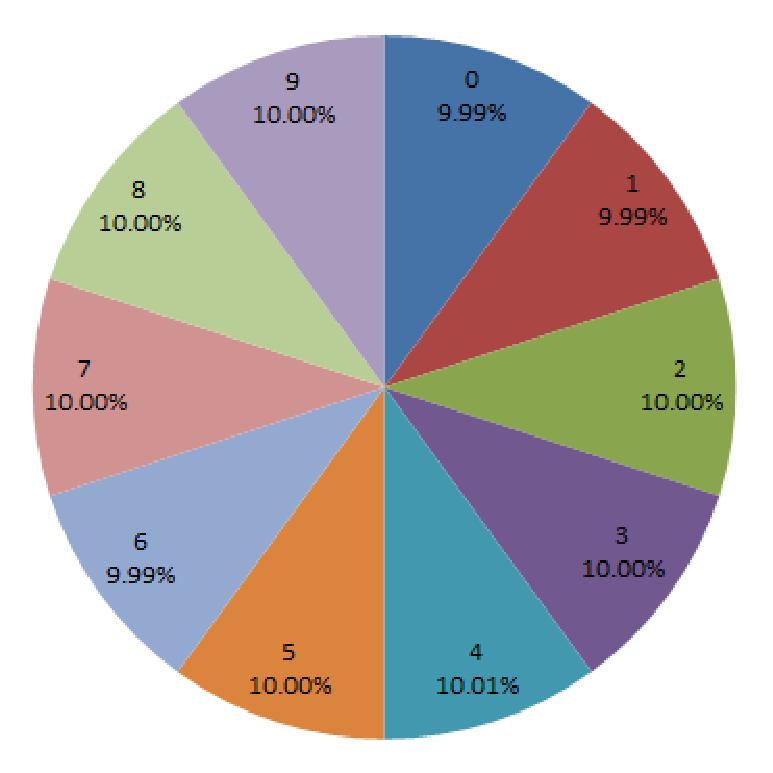
\includegraphics[width=0.9\textwidth,height=7cm]{figures/pipie}
    \end{minipage}
    \begin{minipage}[t]{0.5\linewidth}
        \centering
          
\includegraphics[width=0.9\textwidth,height=7cm]{figures/imrs-pi}
    \end{minipage}
    \caption{圆周率$\pi$值前1,000万位小数所含数字统计图(左)数字一阶转移概率矩阵图(右)}\label{fig:pipie}
\end{figure}

目前,我们还无法完全从理论上证明$\pi$的正则性,根据统计结果数字基本服从均匀分布
\[
    P_i \approx \frac{1}{10} = 0.1, i = 0, 1,\ldots,9,
\]
数值计算几乎可以肯定$\pi$就是一个正则数。如果将每个数字当作一个状态,我们利用$\pi$小数部分相邻数字建立各状态之间的\textbf{一阶转移概率矩阵}$A=(a_{ij})_{10\times 10}$,如图\ref{fig:pipie}(右):
\[
A=
\begin{pmatrix}
    0.0997 & 0.1001 & 0.1002 & 0.0997 & 0.1003 & 0.1000 & 0.0995 & 0.0996 & 0.1009 & 0.0999\\
    0.1005 & 0.0997 & 0.0997 & 0.1003 & 0.1003 & 0.0997 & 0.0997 & 0.0997 & 0.1001 & 0.1001\\
    0.1001 & 0.1003 & 0.1000 & 0.0999 & 0.1000 & 0.1000 & 0.1001 & 0.1003 & 0.0997 & 0.1005\\
    0.1001 & 0.0998 & 0.0994 & 0.1006 & 0.1001 & 0.1000 & 0.1001 & 0.0997 & 0.1001 & 0.1007\\
    0.1003 & 0.1003 & 0.1003 & 0.0998 & 0.1000 & 0.1002 & 0.1004 & 0.1004 & 0.1001 & 0.1000\\
    0.1002 & 0.1002 & 0.0999 & 0.0998 & 0.1001 & 0.1005 & 0.1000 & 0.1005 & 0.0996 & 0.1002\\
    0.0998 & 0.0996 & 0.1007 & 0.1001 & 0.1005 & 0.1000 & 0.1000 & 0.0997 & 0.0999 & 0.0997\\
    0.0994 & 0.1005 & 0.1001 & 0.1005 & 0.1000 & 0.1001 & 0.1001 & 0.1003 & 0.0998 & 0.1000\\
    0.1000 & 0.0998 & 0.1003 & 0.1000 & 0.1001 & 0.1004 & 0.1003 & 0.1003 & 0.0998 & 0.0994\\
    0.0999 & 0.0997 & 0.1003 & 0.0998 & 0.1004 & 0.1000 & 0.0997 & 0.1003 & 0.1004 & 0.1001
\end{pmatrix}
\]
转移矩阵的每一项表示一个状态转移概率
\[
    P(\pi_t = i|\pi_{t+1} = j)\approx 0.1,~~~i,j = 0,1,2,\ldots,9,
\]
每个状态都是近似于随机跳转。
\end{example}

\begin{definition}[二项分布]
如果记$A$为一次成功的伯努利实验,$p$为事件$A$发生的概率,$X$为$n$重伯努利实验中成功的次数,则$X$的可能取值为$0,1,\ldots,n$,随机变量$X$的分布列为
\begin{equation}
    P(X=k) = \binom{n}{k} p^k (1-p)^{n-k}
\end{equation}
则称$X$服从\textbf{二项分布}(Binomial Distribution),写作$X\sim B(n,p)$。当$n=1$时,则称$X$服从\textbf{两点分布},或称\textbf{$0-1$分布}:
\begin{equation}
    P(X=k) = p^k (1-p)^{1-k}, \quad k = 0, 1
\end{equation}
\end{definition}

\begin{definition}[几何分布]
如果记$A$为一次成功的伯努利实验,$p$为事件$A$发生的概率,$X$为重复伯努利实验直至事件$A$发生所需的实验次数,则$X$的可能取值为$1,\ldots,n$,随机变量$X$ 的分布列为
\begin{equation}
    P(X=k) = (1-p)^{k-1} p,\quad k = 1,2,\ldots
\end{equation}
则称$X$服从\textbf{几何分布}(Geometric Distribution),写作$X\sim \mathrm{Geo}(p)$。
\end{definition}

\begin{theorem}[几何分布的无记忆性]
假设$X\sim \mathrm{Geo}(p)$,则对任意正整数$m$与$n$,都有
\begin{equation}
    P(X > m + n | X > m) = P(X > n).
\end{equation}
\end{theorem}

\begin{definition}[负二项分布]
如果记$A$为一次成功的伯努利实验,$p$为事件$A$发生的概率,$X$为重复伯努利实验直至事件$A$出现$r$次所需的实验次数,则$X$的可能取值为$r,r+1,\ldots$,随机变量$X$ 的分布列为
\begin{equation}
    P(X=k) = \binom{k-1}{r-1} p^r (1-p)^{k-r},\quad k = r,r+1,\ldots,
\end{equation}
则称$X$服从\textbf{负二项分布}(Negative Binomial Distribution)或\textbf{Pascal分布},写作$X\sim \textrm{NB}(r, p)$。当$r=1$时,退化为几何分布。
\end{definition}

\begin{definition}[超几何分布]
假设有$N$个产品,其中有$M$个不合格产品。如果无放回地从中随机抽取$n$个,记$X$为抽取的$n$个产品中不合格的产品数目,则随机变量$X$ 的分布列为
\begin{equation}
    P(X=k) = \dfrac{\binom{M}{k}\binom{N-M}{n-k}}{\binom{N}{n}},\quad k = 1,2,\ldots, r
\end{equation}
则称$X$服从\textbf{超几何分布}(Hypergeometric Distribution),即$X\sim \mathrm{HGeo}(n, N, M)$,其中$r=\min~\{M,n\}$,并满足$M\le N$,$n\le N$,$n,M,N\in \mathbb N^{+}$。
\end{definition}

\begin{definition}[泊松分布]
如果随机变量$X$的分布列为
\begin{equation}
    P(X=k) = \frac{\lambda^k}{k!} e^{-\lambda},\quad k = 0,1,\ldots
\end{equation}
则称$X$服从\textbf{泊松分布}(Poisson Distribution),写作$X\sim \mathrm{Po}(\lambda)$。
\end{definition}

泊松分布是法国数学家Sim\'{e}on-Denis Poisson于1837年首次公开的一种离散型概率分布,它适合于刻画单位时间(或单位空间、单位产品)上随机事件发生的次数(计数过程),比如某一服务设施在一定时间内到达的人数,电话交换机接到呼叫的次数,汽车站台的候客人数,机器出现的故障数,自然灾害发生的次数,一块产品上的缺陷数,显微镜下单位分区细菌分布的数目等。

\begin{definition}[均匀分布]
如果随机变量$X$的概率密度函数为
\begin{equation}
    f(x;a, b) = \left\{
        \begin{array}{rl}
          \frac{1}{b-a}, & a < x < b, \\
          0, & else.
        \end{array}
        \right.
\end{equation}
则称$X$服从区间$(a,b)$上的\textbf{均匀分布}(Uniform Distribution),写作$X\sim U(a,b)$。
\end{definition}

\begin{definition}[指数分布]
如果随机变量$X$的概率密度函数为
\begin{equation}
    f(x;\lambda) = \left\{
        \begin{array}{rl}
          \lambda e^{-\lambda x}, & x \ge 0, \\
          0, & x < 0.
        \end{array}
        \right.
\end{equation}
则称$X$服从\textbf{指数分布}(Exponential Distribution),写作$X\sim \mathrm{Exp}(\lambda)$,$\lambda>0$为率参数(Rate Parameter),表示在单位时间间隔随机事件发生的次数。
\end{definition}

\begin{theorem}[指数分布的无记忆性]
如果$X\sim E(\lambda)$,则对任意的$s,t>0$,都有
\begin{equation}
    P(X > s+t | X>s) = P(X>t).
\end{equation}
\end{theorem}

\begin{definition}[正态分布]
如果随机变量$X$的概率密度函数为
\begin{equation}
    f(x;\mu,\sigma) = \frac{1}{\sqrt{2\pi}\sigma} \exp\{-\frac{(x-\mu)^2}{2\sigma^2}\},\quad x\in (-\infty,\infty)
\end{equation}
则称$X$服从\textbf{正态分布}(Normal Distribution),也称\textbf{高斯分布}(Gaussian Distribution)或\textbf{钟形分布}(Bell Distribution),记作$X\sim N(\mu,\sigma^2)$,参数$\mu,\sigma$ 分别表示变量的均值与标准差。当$\mu=0$,$\sigma=1$时,$X$服从\textbf{标准正态分布}$N(0,1)$。
\end{definition}

\begin{corollary}
如果随机变量$X\sim N(\mu,\sigma)$,则随机变量$Z=\frac{X-\mu}{\sigma}\sim N(0,1)$。
\end{corollary}
\begin{proof}
根据连续变量分布函数的定义,对于任意的$z\in \mathbb R$,$Z$的分布函数可表示如下:
\[
    F(z) = P(Z\le z) = P(\frac{X-\mu}{\sigma} \le z) = P(X \le \mu + z\sigma)=\int_{-\infty}^{\mu + z\sigma} f(x;\mu,\sigma) dx,
\]
展开可知
\[
    F(z) = \int_{-\infty}^{\mu + z\sigma} \frac{1}{\sqrt{2\pi}\sigma} \exp\{-\frac{(x-\mu)^2}{2\sigma^2}\} dx = \int_{-\infty}^z \frac{1}{\sqrt{2\pi}} \exp\{-\frac{x^2}{2}\} dx,
\]
直接求导可以得到相应的概率密度函数
\[
    f(z) = \frac{1}{\sqrt{2\pi}} \exp\{-\frac{x^2}{2}\},
\]
由此证得$Z\sim N(0,1)$。
\end{proof}

如果随机变量$X\sim N(\mu,\sigma)$,我们现在分析概率密度函数的凹凸性,对它求二次导数:
\[
    \frac{\partial f(x;\mu,\sigma)}{\partial x} = \frac{1}{\sqrt{2\pi} \sigma} \exp\{-\frac{(x-\mu)^2}{2\sigma^2}\} \frac{1}{\sigma^2} [\frac{(x-\mu)^2}{\sigma^2} - 1],
\]
由此可知$f(x;\mu,\sigma)$的拐点在$x=\mu \pm\sigma$处,当$|x|<\mu +\sigma$时,$f(x;\mu,\sigma)$是凹函数,否则$f(x;\mu,\sigma)$是凸函数。此外,所有正态分布都遵循一个3$\sigma$原则:$P(|x-\mu|\le \sigma) = 68.27\%$,$P(|x-\mu|\le 2\sigma) = 95.45\%$,$P(|x-\mu|\le 3\sigma) = 99.7\%$,可以方便日常估算。

\begin{theorem}
如果随机变量$X\sim N(\mu,\sigma)$,则它的数学期望是$\mu$。
\end{theorem}
\begin{proof}
利用连续随机变量的数学期望定义可知
\[
\begin{array}{lcl}
    E(X) &=& \int_{-\infty}^{+\infty}x  f(x;\mu,\sigma) dx\\
    &=& \int_{-\infty}^{+\infty}x  \frac{1}{\sqrt{2\pi}\sigma} \exp\{-\frac{(x-\mu)^2}{2\sigma^2}\} dx\\
    &=& \frac{1}{\sqrt{2\pi}\sigma} \int_{-\infty}^{+\infty} x \exp\{-\frac{(x-\mu)^2}{2\sigma^2}\} dx\\
    &=& \frac{1}{\sqrt{2\pi}} \int_{-\infty}^{+\infty} (x + \mu)\exp\{-\frac{x^2}{2}\} dx\\
    &=& \frac{\mu}{\sqrt{2\pi}} \int_{-\infty}^{+\infty} \exp\{-\frac{x^2}{2}\} dx.
\end{array}
\]
我们利用二重积分,通过极坐标变换
\[
\left\{
    \begin{array}{lcl}
        x &=& r\cos\theta,\\
        y &=& r\sin\theta,
    \end{array}
\right.
\]
简化计算:
\[
\begin{array}{lcl}
    E(X)^2 &=& \frac{\mu^2}{2\pi} \int_{-\infty}^{+\infty} \int_{-\infty}^{+\infty} \exp\{-\frac{x^2 + y^2}{2}\} dx dy\\
    &=& \frac{\mu^2}{2\pi} \int_0^{2\pi} \int_0^{+\infty} r \exp\{-\frac{r^2}{2}\} dr d\theta\\
    &=& \mu^2 [\exp\{-\frac{r^2}{2}\}_{|r=0} - \exp\{-\frac{r^2}{2}\}_{|r=+\infty}]\\
    &=& \mu^2,
\end{array}
\]
由于$E(X)>0$,则$E(X)=\mu$得证。
\end{proof}

\begin{definition}[对数正态分布]
如果随机变量$X$的概率密度函数为
\begin{equation}
    f(x;\mu,\sigma) = \frac{1}{x\sigma\sqrt{2\pi}} \exp\{-\frac{(\ln x-\mu)^2}{2\sigma^2}\},\quad x > 0
\end{equation}
则称$X$服从\textbf{对数正态分布}(Logarithmic Normal Distribution),也称\textbf{高尔顿分布}(Galton Distribution),记作$X\sim \mathrm{LN}(\mu,\sigma^2)$。
\end{definition}

\begin{theorem}
如果$X\sim \mathrm{LogN}(\mu, \sigma^2)$,则$Y=\ln X\sim N(\mu, \sigma^2)$。如果$\sigma>0$,则有\[Z=(Y-\mu)/\sigma\sim N(0,1).\]
\end{theorem}

\begin{definition}[伽马分布]
如果随机变量$X$的概率密度函数为
\begin{equation}
    f(x;\alpha,\lambda) = \left\{
    \begin{array}{cc}
        \frac{\lambda^\alpha}{\Gamma(\alpha)} x^{\alpha-1} e^{-\lambda x} & x \ge 0,\\
        0 & x < 0.
    \end{array}
    \right.
\end{equation}
则称$X$服从\textbf{伽马分布}(Gamma Distribution),记作$X\sim \mathrm{Ga}(\alpha,\lambda)$,其中$\alpha>0$为\textbf{形状参数}(Shape Parameter),$\lambda>0$为\textbf{尺度参数}(Scale Parameter),$\Gamma$ 表示如下形式的伽马函数:
\begin{equation}
    \Gamma(\alpha) = \int_0^{+\infty} x^{\alpha-1} e^{-x} dx,\quad \alpha>0.
\end{equation}
当$\alpha=1$时,伽马分布退化为指数分布,当$\alpha=n/2$,$\lambda=1/2$时,伽马分布退化为自由度为$n$的卡方分布。
\end{definition}

\begin{definition}[贝塔分布]
如果随机变量$X$的概率密度函数为
\begin{equation}
    f(x;a,b) = \left\{
    \begin{array}{rl}
        \frac{1}{B(a,b)} x^{a-1} (1- x)^{b-1}, & 0 < x < 1,\\
        0, & else.
    \end{array}
    \right.
\end{equation}
则称$X$服从\textbf{贝塔分布}(Beta Distribution),记作$X\sim \mathrm{Be}(a,b)$,其中$a,b>0$都是形状参数,$B$表示如下形式的贝塔函数:
\begin{equation}
    B(a,b) = \int_0^1 x^{a-1} (1-x)^{b-1} dx,\quad a>0,b>0.
\end{equation}
根据伽马函数的定义可知两者存在下面形式的关系:
\begin{equation}
    B(a,b) = \frac{\Gamma(a)\Gamma(b)}{\Gamma(a+b)}.
\end{equation}
当$a=b=1$时,贝塔分布退化为均匀分布$U(0,1)$。
\end{definition}

\begin{definition}[拉普拉斯分布]
如果随机变量$X$的概率密度函数为
\begin{equation}
    f(x;\eta,\theta) = \frac{1}{2\theta} \exp\{-\frac{|x-\eta|}{\theta}\},\quad x \in (-\infty,\infty)
\end{equation}
则称$X$服从\textbf{拉普拉斯分布}(Laplace Distribution),也称\textbf{双指数分布},记作$X\sim \mathrm{La}(\eta,\theta)$,参数$\eta,\theta$分别表示随机变量$X$ 的均值与标准差。
\end{definition}

1901年,Josiah Gibbs在研究统计力学时发现一种新的分布模型:\textbf{玻尔兹曼分布}(Boltzmann Distribution),也称\textbf{Gibbs分布}。在统计和机器学习领域,玻尔兹曼分布又称作\textbf{对数线性模型}(Log-linear Model)。
\begin{definition}[玻尔兹曼分布]
在一个封闭系统中,当系统温度为$T$时,处于状态$S_i$,能量为$E_i$的粒子所占比例$N_i/N$
\begin{equation}
    \frac{N_i}{N} = \frac{1}{Z(T)} g_i \exp\{-\frac{E_i}{\kappa T}\}
\end{equation}
其中,$g_i$表示拥有能量$E_i$的状态数目,$Z(T)$是标准化因子,在统计力学中称\textbf{配分函数(Partition Function)}
\begin{equation}
    Z(T) = \sum\limits_i g_i \exp\{-\frac{E_i}{\kappa T}\}
\end{equation}
而$N$表示系统中粒子总数$N=\sum\limits_i N_i$。
\end{definition}

\begin{theorem}[卷积公式]
假设$X$与$Y$是两个相互独立的连续型随机变量,两变量的概率密度函数分别是$f_X(x)$和$f_Y(y)$,则两者之和$Z=X+Y$的概率密度函数为
\begin{equation}
    f_Z(z) = \int_{-\infty}^{+\infty} f_X(z-y) f_Y(y) dy
\end{equation}
也称概率密度函数$f_X(x)$和$f_Y(y)$的\textbf{卷积}(Convolution),可视作\textbf{移动平均}的推广。
\end{theorem}

\begin{theorem}[正态分布的可加性]
假设$X\sim N(\mu_1,\sigma_1^2)$,$Y\sim N(\mu_2,\sigma_2^2)$,且相互独立,则$Z=X+Y\sim N(\mu_1+\mu_2,\sigma_1^2 +\sigma_2^2)$。
\end{theorem}

\section{概率不等式}%Probability Inequalities
\subsection{集中不等式}
集中不等式(Concentration Inequalities)刻画了一个随机变量在给定取值附近集中分布的状况。比如,大数定律描述了一系列独立同分布随机变量的均值在概率上趋近于它们的数学期望。当变量数目逐渐增大,变量均值会集中在变量期望附近。

\begin{theorem}[Markov不等式]
假设$X$是非负随机变量,存在期望$E(X)$。对于任意的实数$t>0$,都有
\begin{equation}
    P(X\ge t) \le \frac{E(X)}{t}
\end{equation}
\end{theorem}
\begin{proof}
记变量
\begin{equation}
    I = \left\{
        \begin{array}{ll}
          1 & X\ge t \\
          0 & X < t
        \end{array}
    \right.
\end{equation}
由于$I\le X/t$,两边同时取期望,则有$P(X\ge t)=E(I) \le E(X)/t$成立。
\end{proof}

\begin{theorem}[Mill不等式]
假设随机变量$X\sim N(0,1)$,则对任意的实数$t>0$,都有
\[
    P(|X|>t) \le \sqrt{\frac{2}{\pi}} \frac{e^{-t^2/2}}{t}.
\]
\end{theorem}
\begin{proof}
根据定义则有
\[
\begin{array}{lcl}
    P(|X|>t) &=& \int_{-\infty}^{-t} f(x) dx + \int_t^{+\infty} f(x) dx \\
    &=& 2\int_t^{+\infty} \frac{1}{\sqrt{2\pi}} e^{-x^2/2} dx\\
    &\le& \sqrt{\frac{2}{\pi}} \int_t^{+\infty} \frac{x}{t} e^{-x^2/2} dx\\
    &=& \sqrt{\frac{2}{\pi}} \frac{e^{-t^2/2}}{t}.
\end{array}
\]
证毕。
\end{proof}

\begin{theorem}[Chebyshev不等式]
假设随机变量$X$存在期望$\mu = E(X)$和方差$\sigma^2 = \var(X)$,则对任意的实数$t>0$,都有
\begin{equation}
    P(|X-\mu|\ge t) \le \frac{\sigma^2}{t^2}
\end{equation}
\end{theorem}
\begin{proof}
由于$(X-\mu)^2$是非负随机变量,由Markov不等式可知
\begin{equation}
    P((X-\mu)^2\ge t^2) \le \frac{E[(X-\mu)^2]}{t^2} = \frac{\sigma^2}{t^2}
\end{equation}
等价于
\begin{equation}
    P(|X-\mu|\ge t) \le \frac{\sigma^2}{t^2}
\end{equation}
若记$Z = (X-\mu)/\sigma$,则有
\begin{equation}
    P(|Z|\ge 2) \le \frac{1}{4}, ~~P(|Z|\ge 3) \le \frac{1}{9}
\end{equation}
Chebyshev不等式并未限定随机变量分布的具体形式,存在广泛应用。
\end{proof}

\begin{theorem}[Chernoff界]
如果随机变量$X$存在矩母函数$\psi$,则对任意的$t$,都有
\[
    P(X\ge t) \le \min\limits_{s>0} \frac{\psi(s)}{e^{st}}.
\]
\end{theorem}
\begin{proof}
对于任意的$s>0$,都有
\[
    P(X\ge t) = P(e^{sX} \ge e^{st}),
\]
根据Markov不等式可得
\[
    P(e^{sX} \ge e^{st}) \le e^{-st} E(e^{sX} = \frac{\psi(s)}{e^{st}}.
\]
由于$s$的任意性,从而可得
\[
    P(X\ge t) \le \min\limits_{s>0} \frac{\psi(s)}{e^{st}}.
\]
\end{proof}

\begin{lemma}[Hoeffding法则]
假设$X$是$[a,b]$上的随机变量,并且$E(X)=0$,则对任意实数$t>0$有
\begin{equation}
   \psi(t) = E[e^{tX}] \le e^{t^2(b-a)^2/8}
\end{equation}
\end{lemma}
\begin{proof}
由于$e^{tX}$是凸函数,则由Jensen不等式可知
\begin{equation}
  e^{tX} \le \frac{b-X}{b-a} e^{ta} + \frac{X-a}{b-a} e^{tb}
\end{equation}
两边同时取期望,则有
\begin{equation}
  E[e^{tX}] \le \frac{E(b-X)}{b-a} e^{ta} + \frac{E(X-a)}{b-a} e^{tb}
\end{equation}
由于$E(X)=0$,所以
\begin{equation}
  E[e^{tX}] \le \frac{b}{b-a} e^{ta} - \frac{a}{b-a} e^{tb} \triangleq e^{\phi(t)}
\end{equation}
其中,$\phi(t)=\ln\big(\frac{b}{b-a} e^{ta} - \frac{a}{b-a} e^{tb}\big)$,我们只要证明$\phi(t)\le t^2(b-a)^2/8$即可。

由于
\begin{eqnarray}
    \phi'(t) &=& \frac{ab}{b e^{ta} - a e^{tb}} (e^{ta} - e^{tb}) \\
    \phi''(t) &=& \frac{(1-\alpha) e^{-t(b-a)}}{[(1-\alpha) e^{-t(b-a)} + \alpha]} \times \frac{\alpha}{[(1-\alpha) e^{-t(b-a)} + \alpha]} \times (b-a)^2 \le \frac{1}{4} (b-a)^2,
    \end{eqnarray}
其中,$\alpha=\frac{-a}{b-a}$。根据Taylor展开式,可知存在$\theta\in[0,t]$,满足
\begin{equation}
  \phi(t) = \phi(0) + t\phi'(0) + \frac{1}{2} t^2 \phi''(\theta) \le \frac{1}{8} t^2(b-a)^2
\end{equation}
则命题得证。
\end{proof}

\begin{theorem}[Hoeffding不等式]
假设$X_1,\ldots, X_n$是相互独立的随机变量,且$X_i\in[a_i,b_i], i =1,\ldots,n$。记$S_n=\sum\limits_i X_i$,对任意的$\epsilon>0$则有
\begin{equation}
    P(|S_n-E(S_n)| \ge \epsilon) \le \exp\bigg\{-\frac{2\epsilon^2}{\sum\limits_i (b_i-a_i)^2}\bigg\}.
\end{equation}

\begin{proof}
由于$P(S_n-E(S_n) \ge \epsilon) = P(e^{S_m-E(S_m)} \ge e^\epsilon)$,根据Markov不等式,则有
\begin{equation}
    P(e^{t[S_n-E(S_n)]} \ge e^{t\epsilon}) \le \frac{E[e^{t
    [S_n-E(S_n)]}]}{e^{t\epsilon}} = \frac{E[\prod\limits_i e^{t(X_i-E(X_i))}]}{e^{t\epsilon}}
\end{equation}
由$X_1,X_2,\ldots, X_n$的独立性和Hoeffding法则有
\begin{equation}
  \frac{E[\prod\limits_i e^{t(X_i-E(X_i))}]}{e^{t\epsilon}} = \frac{\prod\limits_i E[e^{t(X_i-E(X_i))}]}{e^{t\epsilon}} \le \frac{\prod\limits_i e^{t^2(b_i-a_i)^2/8}}{e^{t\epsilon}} = \frac{e^{t^2 \sum\limits_i (b_i-a_i)^2/8}}{e^{t\epsilon}}
\end{equation}
只要取$t = 4\epsilon/\sum\limits_i (b_i-a_i)^2$,则
\begin{equation}
    P(S_m-E(S_m) \ge \epsilon) \le \exp\bigg\{-\frac{2\epsilon^2}{\sum\limits_i (b_i-a_i)^2}\bigg\},
\end{equation}
同理可证
\begin{equation}
    P(S_m-E(S_m) \le -\epsilon) \le \exp\bigg\{-\frac{2\epsilon^2}{\sum\limits_i (b_i-a_i)^2}\bigg\},
\end{equation}
命题得证。
\end{proof}
\end{theorem}
Hoeffding不等式从本质上说明一组独立随机变量的均值离开其期望值的可能性以指数形式衰减,即有
\[
    P(|\bar X - E (\bar X)| \ge \epsilon) \le \exp\bigg\{-\frac{2 n^2 \epsilon^2}{\sum\limits_i (b_i-a_i)^2}\bigg\}\rightarrow 0~~~(n\rightarrow \infty).
\]
如果每个随机变量都有一个较小的方差,我们可以推导出更紧的概率界。

\begin{lemma}[Azuma法则]
假设随机变量$X$和$Y$满足$E(X|Y)=0$,且存在函数$f$和常数$c$使得不等式$f(Y)\le X \le f(Y)+c$成立,则对任意的实数$t>0$都有
\begin{equation}
    E(e^{tX}|Y) \le \exp\{\frac{t^2c^2}{8}\}.
\end{equation}

\end{lemma}
\begin{proof}
根据Hoeffding法则与条件期望的相加性,命题易证。我们令$a = f(Y)$,$b = f(Y) + c$,于是$b - a = c$。由于$e^{tX}$是凸函数,则由Jensen不等式可知
\begin{equation}
  e^{tX} \le \frac{b-X}{b-a} e^{ta} + \frac{X-a}{b-a} e^{tb}
\end{equation}
由$E(X|Y)=0$和条件期望的线性相加性可得:
\begin{equation}
    E(e^{tX}|Y) \le E\bigg(\frac{b-X}{b-a} e^{ta} + \frac{a-X}{b-a}e^{tb} |Y\bigg) = \frac{b e^{ta}-a e^{tb}}{b-a}.
\end{equation}
之后证明与Hoeffding不等式的证明完全一致,命题得证。
\end{proof}

\begin{definition}[鞅差序列]
假设$X_1,X_2,\ldots$和$Y_1, Y_2,\ldots$是两个随机变量序列,如果对于任意$i>0$,$Y_i$是$X_1,X_2,\ldots,X_i$的函数,且有
\[
    E(Y_{i+1}|X_1,X_2,\ldots,X_i) = 0,
\]
则称$Y_1, Y_2,\ldots$是关于$X_1,X_2,\ldots$的\textbf{鞅差序列}。
\end{definition}

\begin{theorem}[Azuma不等式]
假设$Y_1, Y_2,\ldots$是关于$X_1,X_2,\ldots$的鞅差序列,如果对于任意的$i>0$,都存在常数$c_i$和关于$X_1,X_2,\ldots,X_{i-1}$的随机变量$Z_i$,并满足不等式
$Z_i\le Y_i \le Z_i + c_i$,那么对任意的$\epsilon>0$和正整数$n$都有
\[
    P(|\sum\limits_n Y_i| \ge \epsilon) \le \exp\big\{-\frac{2\epsilon^2}{\sum\limits_i c_i^2}\big\}.
\]
\end{theorem}

\begin{proof}
假设$S_k=\sum\limits_{i=1}^k Y_i$,$1\le k\le n$,则对任意的实数$t>0$,由Markov不等式易知
\[
    P(S_n\ge \epsilon) = P(tS_n\ge t\epsilon) \le \frac{E e^{tS_n}}{e^{t\epsilon}} = \frac{E (e^{tS_{n-1}} e^{tY_n})}{e^{t\epsilon}},
\]
并且$e^{tS_{n-1}}$是$X_1,X_2,\ldots,X_{n-1}$的函数,由条件期望的性质可得
\[
    E (e^{tS_{n-1}} e^{tY_n}) = E\big(e^{tS_{n-1}} E(e^{tY_n}|X_1,X_2,\ldots, X_{n-1})\big).
\]
根据Azuma法则可知$E(e^{tY_n}|X_1,X_2,\ldots, X_{n-1}) \le e^{t^2 c_n^2/8}$,于是有
\[
    P(S_n\ge \epsilon) \le \frac{E (e^{tS_{n-1}} e^{tY_n})}{e^{t\epsilon}} \le \frac{E (e^{tS_{n-1}} e^{t^2 c_n^2/8})}{e^{t\epsilon}} \le \cdots \le \frac{e^{t^2 \sum\limits_i c_i^2/8}}{e^{t\epsilon}}.
\]
如果取$t=4\epsilon /\sum\limits_i c_i^2$,可得
\[
    P(\sum\limits_i Y_i \ge \epsilon) \le \exp\big\{-\frac{2\epsilon^2}{\sum\limits_i c_i^2}\big\},
\]
同理可证
\[
    P(\sum\limits_i Y_i \le -\epsilon) \le \exp\big\{-\frac{2\epsilon^2}{\sum\limits_i c_i^2}\big\},
\]
命题得证。
\end{proof}

\begin{theorem}[McDiarmid不等式]
假设$X_1,\ldots, X_n\in \mathcal X$是相互独立的随机变量且存在实数$c_1,\ldots,c_n>0$和函数$f:\mathcal X^n \mapsto \mathbb R$,使得对于任意的$x_1,\ldots,x_i, \ldots, x_n,x'_i$都有
\[
   |f(x_1,\ldots,x_i,\ldots,x_n) - f(x_1,\ldots,x'_i,\ldots,x_n)| \le c_i,
\]
设$f(S)=f(X_1,X_2,\ldots, X_n)$,那么对于任意的$\epsilon>0$和正整数$n$有
\begin{equation}
    P(|f(S) - E(f(S))|\ge \epsilon) \le \exp\big\{-\frac{2\epsilon^2}{\sum\limits_i c_i^2}\big\}.
\end{equation}
\end{theorem}
\begin{proof}
我们记随机变量$Y=f(S)-E(f(S))$和随机变量序列$\{Y_k\}_{k=1}^n$:
\begin{eqnarray}
  \nonumber Y_1 &=& E(Y|X_1) - E(Y), \\
  \nonumber \vdots && \\
  \nonumber Y_k &=& E(Y|X_1, X_2,\ldots,X_k) - E(Y|X_1,X_2,\ldots, X_{k-1}),~~~k=2,3,\ldots,n,
\end{eqnarray}
显然$\sum\limits_k Y_k = E(Y|X_1, X_2,\ldots,X_n) - E(Y)$,又$E(Y)=0$,而
\[
\begin{array}{lcl}
    E(Y|X_1, X_2,\ldots,X_n) &= &E(f(S)-E(f(S))|X_1, X_2,\ldots,X_n)\\
     &=& E(f(S)|X_1, X_2,\ldots,X_n) - E(E(f(S))|X_1, X_2,\ldots,X_n),
\end{array}
\]
由于$f(S)$是$X_1,X_2,\ldots, X_n$的一个函数,$E(f(S))$是个标量,所以有
\[
    \sum\limits_k Y_k = E(Y|X_1, X_2,\ldots,X_n) = f(S) - E(f(S)) = Y.
\]
此外,根据条件期望的性质可知
\[
    E(Y|X_1,\ldots,X_k) = E(E(Y|X_1,\ldots,X_k)|X_1,\ldots,X_{k-1}),
\]
于是
\begin{eqnarray}
  \nonumber E(Y_k|X_1,\ldots,X_{k-1}) &=& E(E(Y|X_1, X_2,\ldots,X_k) - E(Y|X_1,X_2,\ldots, X_{k-1})|X_1,\ldots,X_{k-1}) \\
  \nonumber &=&  E(E(Y|X_1, X_2,\ldots,X_k)|X_1,\ldots,X_{k-1}) - \\
  \nonumber &&   E(E(Y|X_1,X_2,\ldots, X_{k-1})|X_1,\ldots,X_{k-1})\\
  \nonumber &=&  E(Y|X_1,\ldots,X_k) - E(Y|X_1,X_2,\ldots, X_{k-1})\\
  \nonumber &=&  0.
\end{eqnarray}
所以序列$Y_1,Y_2,\ldots, Y_n$是关于$X_1,X_2,\ldots, X_n$的鞅差序列。由于$E(f(S))$是个标量,则
\[
    Y_k = E(Y|X_1,\ldots,X_k) - E(Y|X_1,\ldots,X_{k-1}) = E(f(S)|X_1,\ldots,X_k) - E(f(S)|X_1,\ldots,X_{k-1}),
\]
我们定义$U_k$和$V_k$:
\begin{eqnarray}
  \nonumber U_k &=& \sup\limits_X E (f(S) |X_1,\ldots,X_{k-1},X ) - E (f(S) |X_1,\ldots,X_{k-1}), \\
  \nonumber V_k &=& \inf\limits_X E (f(S) |X_1,\ldots,X_{k-1},X ) - E (f(S) |X_1,\ldots,X_{k-1}),
\end{eqnarray}
可知$U_k-V_k=\sup\limits_{X, X'} E (f(S) |X_1,X_2,\ldots,X_{k-1},X ) - E (f(S) |X_1,X_2,\ldots,X_{k-1},X')\le c_k$,从而有不等式
$V_k\le Y_k \le U_k \le V_k + c_k$,由Azuma不等式可得:
\[
    P(f(S) - E(f(S)) \ge \epsilon) \le \exp\big\{-\frac{2\epsilon^2}{\sum\limits_i c_i^2}\big\},
\]
同理可证
\[
    P(f(S) - E(f(S)) \le -\epsilon) \le \exp\big\{-\frac{2\epsilon^2}{\sum\limits_i c_i^2}\big\}.
\]
证毕。
\end{proof}
如果取$f(x_1,x_2,\ldots, x_n) = \sum\limits_i x_i$,可以看出Hoeffiding不等式是McDiarmid不等式的一个特例。

\begin{theorem}[Bennett不等式和Bernstein不等式]
假设随机变量$X_1,X_2,\ldots,X_n$是独立的随机变量,且$X_i\le c$,$E (X_i) = 0$,$E (X_i^2) = \sigma_i^2$。如果记$\sigma^2 = \sum\limits_i \sigma_i^2/n$,那么对任意的实数$\epsilon>0$有
\begin{eqnarray}
  P\big(\sum\limits_i X_i/n \ge \epsilon\big) &\le & \exp\bigg\{-\frac{n\sigma^2}{c^2}f(\frac{\epsilon c}{\sigma^2})\bigg\}, \\
  P\big(\sum\limits_i X_i/n \ge \epsilon\big) &\le & \exp\bigg\{-\frac{n\epsilon^2}{2\sigma^2 + 2\epsilon c/3}\bigg\}.
\end{eqnarray}
其中函数$f(x)=(1+x)\log(1+x)-x$,两个不等式分别称作Bennett不等式和Bernstein不等式。
\end{theorem}

\begin{proof}
对任意实数$t>0$,由Markov不等式和$X_1,X_2,\ldots,X_n$的独立性易知:
\begin{equation}
    P\big(\sum\limits_i X_i/n \ge \epsilon\big) = P\big(e^{t\sum\limits_i X_i} \ge e^{n\epsilon t}\big) \le \frac{E(e^{t\sum\limits_i X_i})}{e^{n\epsilon t}} = \frac{\prod\limits_i E(e^{tX_i})}{e^{n\epsilon t}}.
\end{equation}
我们定义$\mathbb R$上的一个连续函数$g(x)$:
\[
g(x)=\left\{
\begin{array}{rl}
\dfrac{e^x-1-x}{x^2}, & x\in \mathbb R\setminus \{0\},\\
\dfrac{1}{2}, & x = 0.
\end{array}
\right.
\]
可以证明$g(x)$是单调递增函数,那么给定$t>0$,对于任意的$x\le c$都有$g(tx) \le g(tc)$,即是说
\[
    e^{tx} \le 1 + tx + \frac{x^2}{c^2}(e^{tc} - 1 -tc),
\]
根据期望的线性性质,以及$E(X_i)=0$和$E(X_i^2)=\sigma_i^2$可得
\[
    E(e^{tX_i}) \le E\big[1 + tX_i + \frac{X_i^2}{c^2}(e^{tc} - 1 -tc)\big] = 1 + \frac{\sigma_i^2}{c^2}(e^{tc} - 1 -tc) \le e^{\sigma_i^2(e^{tc}-1-tc)/c^2},
\]
于是
\[
    P\big(\sum\limits_i X_i/n \ge \epsilon\big) \le \frac{\prod\limits_i E(e^{tX_i})}{e^{n\epsilon t}} \le \frac{\prod\limits_i e^{\sigma_i^2(e^{tc}-1-tc)/c^2}}{e^{n\epsilon t}} = \frac{e^{\sigma^2(e^{tc}-1-tc)/c^2}}{e^{n\epsilon t}}.
\]
如果取$t=\log(1+(\epsilon c)/\sigma^2)/c$,可以证得Bennett不等式。

我们引入函数
\[
    h(x) = f(x) - \frac{3}{2} \frac{x^2}{x+3},
\]
可以证明$h(x)$是单调递增函数,且$h(0)=0$,所以$h(x)\ge 0$,即$f(x) \ge \frac{3}{2} \frac{x^2}{x+3}$,于是可以证得Bernstein不等式成立。
\end{proof}
这些形式相似的概率不等式描述了一组独立随机变量的均值偏离其期望的概率。如果将每个随机变量看做是某个样本的分类情况,那么通过这些不等式我们可以直接推得泛化误差偏离经验误差的概率,也是统计学习理论分析的基本思路。

\subsection{大数定律}
\textbf{大数定律}(Law of Large Numbers)讨论随机变量和的平均值的收敛情况,是数理统计学中\textbf{参数估计}的理论基础。\textbf{中心极限定理}(Central Limit Theorem)是讨论随机变量序列部分和的分布渐进收敛于正态分布的一组定理,是数理统计学中\textbf{误差分析}的理论基础,指出大量随机变量近似服从正态分布的条件。大数定律和中心极限定理都涉及到随机变量序列的收敛性分析,比如大数定律涉及到\textbf{依概率收敛}(Convergence in Probability),中心极限定理涉及到\textbf{依分布收敛}(Convergence in Distribution)。这些极限定理(Limit Theorems)是概率论的重要内容和数理统计学的基石之一
\footnote{18$\sim$19世纪,极限定理一直是概率论研究的中心课题。Bernoulli大数定律是第一个从数学上被严格证明的概率论定律,由Bernoulli在其1713年出版的《推测术》中详细给出,而“大数定律”这个名称是由Poisson在1837年给出。美籍匈牙利数学家George Polya是第一个在论著中使用“中心极限定理”(1920)术语的人,他还首创了术语“随机游走”(Random Walk,1921)。最初的中心极限定理是关于$n$重Bernoulli试验的,1716年法国数学家Abraham de Moivre讨论了$p=1/2$的情形,随后Pierre-Simon Laplace将其推广到$0<p<1$的情形。从19世纪中叶到20世纪初,一大批著名的前苏联数学家运用严格的、强有力的数学分析工具,如傅里叶变换等,将Bernoulli大数定律、De Moivre-Laplace中心极限定理推广到一般随机变量序列部分和的情形。}。

\begin{definition}[依概率收敛]
假设$\{X_n, n\in \mathbb N\}$是一个随机变量序列,$X$是一个随机变量。如果对任意的$\epsilon>0$,都有
\[
    \lim\limits_{n\rightarrow +\infty} P(|X_n-X|<\epsilon) = 1,
\]
则称$\{X_n, n\in \mathbb N\}$\textbf{依概率收敛}于$X$,记作$X_n \stackrel{P}{\longrightarrow} X$。
\end{definition}

\begin{definition}[几乎处处收敛]
假设$\{X_n, n\in \mathbb N\}$是一个随机变量序列,$X$是一个随机变量。如果
\[
    P(\lim\limits_{n\rightarrow +\infty} X_n = X) = 1,
\]
则称$\{X_n, n\in \mathbb N\}$\textbf{几乎处处收敛}(Almost Surely Converge)或\textbf{以概率1收敛}(Converge with Probability One)于$X$,记作$X_n \stackrel{a.s}{\longrightarrow} X$。
\end{definition}

\begin{definition}[依分布收敛]
假设$\{X_n, n\in \mathbb N\}$是一个随机变量序列,$X$是一个随机变量,$X_n$的分布函数是$F_n(x)$,$X$的分布函数是$F(x)$。如果对$F(x)$的任意连续点$x$,都有
\[
    \lim\limits_{n\rightarrow +\infty} F_n(x) = F(x),~~~n\in \mathbb N,
\]
则称$\{F_n(x), n\in \mathbb N\}$\textbf{弱收敛}于$F(x)$,记作$F_n(x) \stackrel{W}{\longrightarrow} X$,也称$\{X_n, n\in \mathbb N\}$\textbf{依分布收敛}于$X$,记作$X_n \stackrel{L}{\longrightarrow} X$。
\end{definition}

\begin{theorem}[Bernoulli大数定律]
设$\{X_n,n\in \mathbb N\}$是独立的两点分布随机变量序列,$P(X_n=1)=p$,$P(X_n=0)=1-p$,$0<p<1$,记序列前$n$个随机变量的部分和
\[
    S_n = \sum\limits_{i=1}^n X_i,
\]
则$S_n/n\stackrel{P}{\longrightarrow} p$,对任意的$\epsilon>0$都有
\[
   \lim\limits_{n\rightarrow +\infty} P(|\frac{S_n}{n} - p|<\epsilon) = 1.
\]
\end{theorem}
\begin{proof}
由于$S_n\sim B(n,p)$,则$S_n/n$的数学期望和方差都存在,且$E(S_n/n)=p$,$\var(S_n/n)=p(1-p)/n$。根据Chebyshev不等式,对任意的$\epsilon>0$,都有
\[
    1\ge  P(|\frac{S_n}{n} - p|< \epsilon) \ge 1- \frac{\var(S_n/n)}{\epsilon^2} = 1- \frac{p(1-p)}{n\epsilon^2},
\]
当$n\rightarrow +\infty$时,不等式右端趋于$1$:
\[
    \lim\limits_{n\rightarrow +\infty} P(|\frac{S_n}{n} - p|<\epsilon) = \lim\limits_{n\rightarrow +\infty} P(|\frac{1}{n} \sum\limits_{i=1}^n X_i - \frac{1}{n} \sum\limits_{i=1}^n E(X_i)|<\epsilon) = 1,
\]
命题得证。
\end{proof}

\begin{definition}
设$\{X_n, n\in \mathbb N\}$是一个随机变量序列,如果对任意的$\epsilon>0$,都有
\[
    \lim\limits_{n\rightarrow +\infty} P(|\frac{1}{n} \sum\limits_{i=1}^n X_i - \frac{1}{n} \sum\limits_{i=1}^n E(X_i)|<\epsilon) = 1,
\]
则称$\{X_n, n\in \mathbb N\}$服从大数定律。
\end{definition}

\begin{theorem}[Chebyshev大数定律]
设$\{X_n, n\in \mathbb N\}$是一个独立随机变量序列,如果每个随机变量$X_n$的方差存在,且有共同的上界,即$\var(X_n)\le c$,则$\{X_n, n\in \mathbb N\}$服从大数定律。
\end{theorem}

\begin{proof}
由于$\{X_n, n\in \mathbb N\}$相互独立,则部分和均值方差
\[
    \var(\frac{1}{n} \sum\limits_{i=1}^n X_i) = \frac{1}{n^2} \sum\limits_{i=1}^n \var(X_i) \le \frac{c}{n}.
\]
根据Chebyshev不等式,对任意的$\epsilon>0$都有
\[
    \lim\limits_{n\rightarrow +\infty} P(|\frac{1}{n} \sum\limits_{i=1}^n X_i - \frac{1}{n} \sum\limits_{i=1}^n E(X_i)| < \epsilon) \ge  1 - \frac{\var(\sum\limits_{i=1}^n X_i/n)}{\epsilon^2} \ge 1 - \frac{c}{n\epsilon^2}.
\]
当$n\rightarrow +\infty$时,有
\[
    \lim\limits_{n\rightarrow +\infty} P(|\frac{1}{n} \sum\limits_{i=1}^n X_i - \frac{1}{n} \sum\limits_{i=1}^n E(X_i)|<\epsilon) = 1,
\]
命题得证。
\end{proof}
Chebyshev大数定律只要求$\{X_n, n\in \mathbb N\}$相互独立,并不要求它们是同分布的。如果它们是独立同分布,且方差有限,则$\{X_n, n\in \mathbb N\}$必然服从大数定律。Bernoulli大数定律是Chebyshev大数定律的一个特例。此外,根据证明过程可知,只要有
\[
    \frac{1}{n^2} \var(\sum\limits_{i=1}^n X_i) \rightarrow 0(n\rightarrow +\infty),
\]
则大数定律就能成立。这个条件称作“Markov条件”。

\begin{theorem}[Markov大数定律]
设$\{X_n, n\in \mathbb N\}$是一个随机变量序列,那么有
\[
    \lim\limits_{n\rightarrow +\infty}\frac{1}{n^2} \var(\sum\limits_{i=1}^n X_i) = 0,
\]
则$\{X_n, n\in \mathbb N\}$服从大数定律。
\end{theorem}
\begin{proof}
利用Chebyshev不等式易证。
\end{proof}
Markov大数定律对随机变量序列$\{X_n, n\in \mathbb N\}$没有任何同分布、独立性、不相关的假定。Chebyshev大数定律可由Markov大数定律推得。我们知道,一个随机变量的方差存在,则其数学期望一定存在。反之,如果一个随机变量的数学期望存在,则其方差不一定存在。Bernoulli大数定律、Markov大数定律和Chebyshev大数定律都均假定随机变量序列$\{X_n, n\in \mathbb N\}$的方差存在,Khintchine大数定律只是要求序列的数学期望存在。

\begin{theorem}[Khintchine大数定律]%辛钦
设$\{X_n, n\in \mathbb N\}$是一个独立同分布的随机变量序列,如果$X_n$的数学期望存在,则$\{X_n, n\in \mathbb N\}$服从大数定律。
\end{theorem}

\begin{theorem}[Kolmogorov强大数定律]
设$\{X_n, n\in \mathbb N\}$是一个独立同分布的随机变量序列,则$E(|X_n|)<\infty$的充要条件是
\[
    P(\lim\limits_{n\rightarrow +\infty} \big|\frac{1}{n} \sum\limits_{i=1}^n X_i-\frac{1}{n} \sum\limits_{i=1}^n E(X_i)\big|<\epsilon) = 1.
\]
\end{theorem}

\subsection{中心极限定理}%Central Limit Theorem
\begin{theorem}[Linderberg-Levy中心极限定理]
假设$\{X_n,n\in \mathbb N\}$是独立同分布的随机变量序列,且$E(X_i)=\mu$,$\var(X_i)=\sigma^2>0$,如果记
\[
    Z_n = \frac{(X_1 + X_2 + \ldots + X_n) - n\mu}{\sigma \sqrt n},
\]
当$n\rightarrow\infty$时,则有$Z_n\sim N(0,1)$,即是说,对任意的$z\in \mathbb R$,都有
\[
    \lim\limits_{n\rightarrow +\infty} P(Z_n \le z) = \frac{1}{\sqrt{2\pi}}\int_{-\infty}^z e^{-\frac{t^2}{2}}dt.
\]
\end{theorem}
Linderberg-Levy中心极限定理具有广泛应用,它只假设$\{X_n,n\in \mathbb N\}$独立同分布、方差存在,无论具体分布是什么,只要$n$充分大,都可以利用标准正态分布去逼近,说明了正态分布的普遍性。

\begin{theorem}[De Moivre-Laplace极限定理]
假设$\{X_n,n\in \mathbb N\}$是独立两点分布的随机变量序列,且$E(X_i)=p$,$\var(X_i)=pq>0$,如果记
\[
    Z_n = \frac{(X_1 + X_2 + \ldots + X_n) - np}{\sqrt{npq}},
\]
当$n\rightarrow\infty$时,则有$Z_n\sim N(0,1)$。
\end{theorem}
De Moivre-Laplace极限定理是概率论历史上第一个中心极限定理,属于Linderberg-Levy中心极限定理的一个特例。由于$X_1 + X_2 + \ldots + X_n\sim B(n,p)$,也称“二项分布的正态近似”。

Linderberg-Levy中心极限定理是建立在独立同分布的假设条件下,在实际问题中随机变量序列$\{X_n,n\in \mathbb N\}$的独立性很常见,但是同分布的假设相对苛刻。为了使极限分布是正态分布,必须限定$S_n=\sum\limits_{i=1}^n X_i$的各个加和项,使得它们在概率意义下“均匀地小”。假设$\{X_n,n\in \mathbb N\}$是相互独立的随机变量序列,它们具有有限的数学期望和方差:
\[
    E(X_i) = \mu_i,~~~\var(X_i)=\sigma_i^2,~~~i=1,2,\ldots.
\]
我们将随机变量部分和$S_n$进行标准化处理:
\[
    Z_n = \frac{S_n - (\mu_1 + \mu_2 + \ldots + \mu_n)}{B_n} = \sum\limits_{i=1}^n \frac{X_i - \mu_i}{B_n}.
\]
其中$B_n=\var(S_n)$。如果要求$Z_n$中各项“均匀地小”,即对任意的$\tau>0$,要求事件
\[
    A_{ni} = \Big\{\frac{|X_i-\mu_i|}{B_n} > \tau\Big\} = \Big\{|X_i-\mu_i| > \tau B_n\Big\}
\]
发生的可能性小,或直接要求其概率趋于0。为此,我们设定
\[
    \lim\limits_{n\rightarrow +\infty} P(\max\limits_{1\le i \le n} |X_i-\mu_i| > \tau B_n) = 0.
\]
由于
\[
    P(\max\limits_{1\le i \le n} |X_i-\mu_i| > \tau B_n) = P(\bigcup\limits_{i=1}^n (|X_i-\mu_i| > \tau B_n)) \le \sum\limits_{i=1}^n P(|X_i-\mu_i| > \tau B_n),
\]
如果设各个随机变量$X_i$都是连续的,并且对应密度函数是$f_i(x)$,则
\[
\begin{array}{lcl}
    \sum\limits_{i=1}^n P(|X_i-\mu_i| > \tau B_n) &=& \sum\limits_{i=1}^n \int_{|x-\mu_i| > \tau B_n} f_i(x) dx \\
    &\le& \frac{1}{\tau^2 B_n^2} \sum\limits_{i=1}^n \int_{|x-\mu_i| > \tau B_n} (x-\mu_i)^2 f_i(x) dx,
\end{array}
\]
只要对任意的$\tau>0$,有
\begin{equation}\label{eq:linderberg-condition}
    \lim\limits_{n\rightarrow +\infty} \frac{1}{\tau^2 B_n^2} \sum\limits_{i=1}^n \int_{|x-\mu_i| > \tau B_n} (x-\mu_i)^2 f_i(x) dx =0,
\end{equation}
就可保证$Z_n$各加和项“均匀地小”。

\begin{theorem}[Linderberg中心极限定理]
设$\{X_n,n\in \mathbb N\}$是一个独立随机变量序列,如果它满足Linderberg条件(公式\ref{eq:linderberg-condition}),则对任意的$z\in \mathbb R$,有
\[
    \lim\limits_{n\rightarrow +\infty} P(\frac{1}{B_n} \sum\limits_{i=1}^n (X_i-\mu_i) \le z) = \frac{1}{\sqrt{2\pi}}\int_{-\infty}^z e^{-\frac{t^2}{2}}dt.
\]
\end{theorem}
可以证明,如果随机变量序列是独立同分布、方差有限的序列,则它一定满足Linderberg条件,则Linderberg-Levy中心极限定理与De Moivre-Laplace极限定理都是Linderberg中心极限定理的特例。此外,一般性的Linderberg条件在实际使用时不易验证,Lyapunov中心极限定理提出更容易验证的Lyapunov条件。

\begin{theorem}[Lyapunov中心极限定理]
设$\{X_n,n\in \mathbb N\}$是一个独立随机变量序列,如果存在$\delta>0$,满足\textbf{Lyapunov条件}
\begin{equation}\label{eq:Lyapunov-condition}
    \lim\limits_{n\rightarrow +\infty} \frac{1}{B_n^{2+\delta}} \sum\limits_{i=1}^n  E(|X_i-\mu_i|^{2+\delta}) =0,
\end{equation}
则对任意的$z\in \mathbb R$,有
\[
   \lim\limits_{n\rightarrow +\infty} P(\frac{1}{B_n} \sum\limits_{i=1}^n (X_i-\mu_i) \le z) = \frac{1}{\sqrt{2\pi}}\int_{-\infty}^z e^{-\frac{t^2}{2}}dt.
\]
\end{theorem}

\section{统计与抽样分布}
前面几节属于概率论的范畴,一切计算和推理都是建立在随机变量概率分布已知的假定之上。在处理实际问题时,往往需要收集和整理复杂多样的数据,并借助一些高级的分析方法进行推断和预测,这些就是统计学主要的工作内容。

在统计问题中,我们把统计分析研究对象的全体称作\textbf{总体}(Population),而构成总体的每个成员称作\textbf{个体}(Individual)。总体隐含一个内在的概率分布,统计学期望了解总体的潜在分布,利用抽样技术从总体中随机抽取\textbf{样本}(Sample),根据样本统计特征深化对样本总体的了解。为了能够通过样本对总体做出比较可靠的推断,我们希望样本能够很好地代表总体,一般地会对抽样技术提出一些要求,保证样本的\textbf{随机性}和\textbf{独立性}等性质。

\begin{definition}[统计量]
假设$x_1,x_2,\ldots,x_n$是取自某总体的样本,如果样本函数$T=T(x_1,x_2,\ldots, x_n)$中不含任何未知参数,则称$T$为\textbf{统计量},统计量的分布称作
\textbf{抽样分布}(Sample Distribution)。
\end{definition}

\begin{definition}[样本均值]
假设$x_1,x_2,\ldots,x_n$是取自某总体的样本,其算术平均值称作称作\textbf{样本均值}(Sample Mean),一般记作$\bar x$,则有
\begin{equation}
    \bar x = \frac{1}{n} \sum\limits_i  x_i.
\end{equation}
\end{definition}

\begin{theorem}
假设$x_1,x_2,\ldots,x_n$是取自某总体的样本,则样本数据与样本均值的偏差平方和最小,对任意的$\alpha\in \mathbb R$,都有
\[
    \sum\limits_i (x_i - \bar x)^2 \le \sum\limits_i (x_i - \alpha)^2.
\]
\end{theorem}

\begin{theorem}
假设$x_1,x_2,\ldots,x_n$是取自某总体的样本,(甲)如果总体分布是$N(\mu,\sigma^2)$,则样本均值$\bar x\sim N(\mu,\sigma^2/n)$;(乙)如果总体分布未知或总体分布不是正态分布,但是$E(x)=\mu,\var(x) = \sigma^2$,则当$n$较大时,$\bar x$的\textbf{渐近分布}是$N(\mu,\sigma^2)$,记作:$\bar x \stackrel{\bullet}{\sim} N(0,1)$。
\end{theorem}

\begin{theorem}
设总体$X$具有二阶矩,即$E(X)=\mu$,$\var(X)=\sigma^2 < +\infty$,$x_1,x_2,\ldots,x_n$是从总体$X$抽取的样本,$\bar x$和$s^2$分别是样本均值和样本方差,则有$E(\bar x)=\mu$,$\var(\bar x)=\sigma^2/n$,$E(s^2)=\sigma^2$。
\end{theorem}

\begin{definition}[样本方差和标准差]
假设$x_1,x_2,\ldots,x_n$是取自某总体的样本,则它关于样本均值$\bar x$的偏差平方和
\begin{equation}
    s^2 = \frac{1}{n}\sum\limits_i (x_i - \bar{x}_i)^2
\end{equation}
称为\textbf{有偏样本方差}(Biased Sample Variance),其算术平方根$s$称为\textbf{样本标准差}(Standard Deviation)。在许多应用场合,样本量很小,通常使用如下公式计算\textbf{无偏样本方差}(Unbiased Sample Variance)与标准差
\footnote{无偏样本方差中$1/(n-1)$项称作\textbf{Bessel校正},而$n-1$称作偏差平方和的\textbf{自由度}(Degree of Freedom):当$\bar{x}$确定后,由于条件
$\sum\limits_i (x_i - \bar{x}) = 0$的约束,$n$个偏差$x_1-\bar{x},\ldots,x_n-\bar{x}$中只有$n-1$个数据可以自由变动,总有一个偏差不能自由取值。}:
\begin{equation}
    s^2 = \frac{1}{n-1}\sum\limits_i (x_i - \bar x_i)^2.
\end{equation}
\end{definition}
如果样本$x_1, x_2, \ldots, x_n$是独立同分布的,并且总体$X$的分布函数是$F(x)$,则样本的联合分布函数可以表示如下:
\[
    F(x_1,x_2,\ldots, x_n) = \prod\limits_i F(x_i).
\]

\begin{definition}[次序统计量]
假设$X_1,X_2,\ldots,X_n$是取自总体$X$的样本,$X_{(i)}$称为样本的\textbf{第$i$个次序统计量}(Order Statistic),其取值是将样本观测值由小到大排列后得到的第$i$个观测值,其中$X_{(1)}=\min~\{X_1,X_2,\ldots,X_n\}$称为样本的\textbf{最小次序统计量},$X_{(n)}=\max~\{X_1,X_2,\ldots,X_n\}$称为样本的\textbf{最大次序统计量}。如果对$n$个样本从小到大顺次排列,样本$X_i$在排列中的位置$R_i$称作排名(Rank)。如果$X_i=X_{(1)}$,则有$R_i=1$;如果$X_i=X_{(n)}$,则有$R_i=n$。
\end{definition}
对于一个简单随机样本,$X_1,X_2,\ldots,X_n$独立同分布,次序统计量$X_{(1)},X_{(2)},\ldots,X_{(n)}$既不相互独立,分布也不相同。样本的排名$(R_1, R_2, \ldots, R_n)$是整数$(1,2,\ldots,n)$的一种排列。

\begin{theorem}[单个次序统计量概率分布]
假设总体$X$的概率密度函数为$f(x)$,分布函数为$F(x)$,$X_1,X_2,\ldots,X_n$为样本,则第$i$个次序统计量$X_{(i)}$的概率密度函数为
\begin{equation}
    f_i(x) = \frac{n!}{(i-1)!(n-i)!} [F(x)]^{i-1} [1-F(x)]^{n-i} f(x).
\end{equation}
\end{theorem}

\begin{proof}
根据定义,第$i$个次序统计量$X_{(i)}$的概率分布函数
\begin{eqnarray}
  F(X_{(i)} \le x) & = & P(\text{在$n$个样本观测值中至少有$i$个不大于$x$}) \\
   &=& \sum\limits_{k=i}^n \binom{n}{k} P(X \le x)^k (1-P(X \le x))^{n-k} \\
   &=& \sum\limits_{k=i}^n \binom{n}{k} F(x)^k (1-F(x))^{n-k}.
\end{eqnarray}
根据概率分布函数,可以确定概率密度函数
\begin{eqnarray}
  f_i(x) & = & \frac{d F(X_{(i)} \le x)}{dx} \\
   &=& \sum\limits_{k=i}^n \binom{n}{k} k F(x)^{k-1} (1-F(x))^{n-k} f(x) - \\
   &&\sum\limits_{k=i}^n \binom{n}{k} (n-k) F(x)^{k} (1-F(x))^{n-k-1} f(x)\\
   &=& \sum\limits_{k=i}^n \frac{n!}{(k-1)!(n-k)!} F(x)^{k-1} (1-F(x))^{n-k}f(x)- \\
   && \sum\limits_{k=i}^{n-1} \frac{n!}{k!(n-k-1)!} F(x)^{k} (1-F(x))^{n-k-1}f(x) \\
   &=& \frac{n!}{(i-1)!(n-i)!} F(x)^{i-1} [1-F(x)]^{n-i} f(x).
\end{eqnarray}
\end{proof}

\begin{theorem}[序偶次序统计量概率分布]
假设总体$X$的概率密度函数为$f(x)$,分布函数为$F(x)$,$X_1,X_2,\ldots,X_n$为样本,则序偶次序统计量$(X_{(i)},X_{(j)}), i < j$的联合分布概率密度函数为
\begin{equation}
    f_{ij}(y,z) = \frac{n!}{(i-1)!(j-i-1)!(n-j)!} [F(y)]^{i-1} [F(z)-F(y)]^{j-i-1} [1-F(z)]^{n-j} f(y)f(z),\quad y \le z.
\end{equation}
\end{theorem}

\begin{theorem}[次序统计量联合概率分布]
假设总体$X$的概率密度函数为$f(x)$,分布函数为$F(x)$,$X_1,X_2,\ldots,X_n$为样本,则统计量$(X_{(1)},X_{(2)},\ldots,X_{(n)})$的联合分布概率密度函数为
\begin{equation}
    f_{\pi}(t_1,t_2,\ldots, t_n) = n! \prod\limits_i f(t_i) I_{t_1\le t_2 \le \ldots \le t_n}.
\end{equation}
\end{theorem}

\begin{theorem}[斯特林近似]
假设
\begin{equation}
    s_n = \frac{1}{2} \log(2\pi) + (n+\frac{1}{2}) \log n - n,
\end{equation}
则有
\begin{equation}
    \lim\limits_{n\rightarrow \infty} |s_n - \log n!| = 0,
\end{equation}
等价于
\begin{equation}
    \lim\limits_{n\rightarrow \infty} \frac{\sqrt{2\pi} n^{n + \frac{1}{2}} e^{-n}}{n!} = 1.
\end{equation}
\end{theorem}

\begin{definition}[样本分位数与中位数]
假设总体$X$概率密度函数为$f(x)$,分布函数为$F(x)$,给定样本$x_1,\ldots,x_n$,则它们的$\alpha$分位数$m_\alpha$定义如下:
\begin{equation}
m_\alpha = \left\{
    \begin{array}{rl}
        x_{\lceil n\alpha \rceil}, & n\alpha\notin \mathbb N^+,\\
        \frac{1}{2} [x_{n\alpha} + x_{n\alpha + 1}], & n\alpha\in \mathbb N^+.
    \end{array}
\right.
\end{equation}
当$\alpha=0.5$时,$\alpha$分位数又称“中位数”。
\end{definition}

\begin{theorem}[$\alpha$分位数渐进概率分布]
假设总体$X$的概率密度函数为$f(x)$,它的$\alpha$分位数为$x_\alpha$,$f(x)$在$x_\alpha$处连续且$f(x_\alpha)>0$,则当$n\rightarrow +\infty$时,样本的$\alpha$分位数$m_\alpha$的渐进分布为
\begin{equation}
    m_\alpha \sim N(x_p, \frac{p(1-p)}{n\times f^2(x_p)}).
\end{equation}
特别地,对于样本中位数,当$n\rightarrow +\infty$时近似地有
\begin{equation}
    m_{0.5} \sim N(x_{0.5}, \frac{1}{4n\times f^2(x_{0.5})}).
\end{equation}
\end{theorem}

由于很多统计推断都基于正态分布假设,以标准正态变量为基石构造出来的三个著名统计量在实际中存在广泛应用。本小节详细介绍三大抽样分布的构造。
\begin{definition}[卡方分布]
假设$\{X_i\}_{i=1}^n$是独立同分布于$N(0,1)$的随机变量序列,则$Y=\sum\limits_i X_i$的分布称为自由度为$n$的卡方分布,记为$Y\sim\chi^2(n)$。
\end{definition}

\begin{definition}[$F$分布]
假设$X_1\sim \chi^2(m)$,$X_2\sim \chi^2(n)$,$X_1$与$X_2$独立,则称$Y=\frac{X_1/m}{X_2/n}$的分布是自由度为$m$与$n$的$F$分布,记为$Y\sim F(m,n)$。
\end{definition}

\begin{definition}[$t$分布\footnote{$t$分布是统计学中一类重要的分布,由英国统计学家William Gosset发现。1899年Gosset开始在一家酿酒厂担任酿酒化学技师,从事试验和数据分析工作。由于Gosset接触的样本容量很小,通过大量的实验数据的积累,他发现$t=\sqrt{n-1}(\bar x-\mu)/s$ 的分布与$N(0,1)$存在细微的差异,前者比$N(0,1)$尾部概率更大(厚尾)。它猜测可能存在一个新的分布族,通过深入研究于1908年以“Student”的笔名发表此项研究成果,后人为此也称$t$分布为“学生分布”。$t$ 分布的发现在统计学历史上具有划时代的意义,打破了正态分布一统天下的局面。}]
假设$X_1\sim N(0,1)$,$X_2\sim \chi^2(n)$,$X_1$与$X_2$独立,则称$Y=\frac{X_1}{\sqrt{X_2/n}}$的分布是自由度为$n$的$t$分布,记为$Y\sim t(n)$。
\end{definition}

\section{随机模型与抽样方法}%Random Simulation and Sampling Methods
对于一些复杂的统计问题,有时很难对各种统计方法进行理论分析。为了评估各种方法的优劣性,比较实用的办法是随机模拟:根据问题的要求与条件构造一系列的随机样本,用它们的样本频率代替对应的概率作统计分析与推断,观察根据这些样本作出推断的正确性。一般随机模拟方法的优点在于计算复杂度不依赖于计算空间的维度,在计算非常高维的积分或多指标求和问题时,随机模拟方法相比传统确定性计算方法优势明显。

\subsection{蒙特卡洛方法}
1946年,Stanislaw Ulam、John von Neumann和Nicholas Metropolis 在Los Alamos Scientific Laboratory工作时发明了一种随机模拟方法:\textbf{蒙特卡罗方法}(Monte Carlo Method)\footnote{随机模拟的灵感来自于博彩,蒙特卡罗即是摩洛哥一家赌场,人们还将组合计算中的一些随机模拟方法称为Las Vegas 方法。}。它是一种以概率统计理论为基础、利用(伪)随机数模拟解决计算问题的数值方法。蒙特卡罗方法在金融工程学、宏观经济学、生物医学、计算物理学等领域都有重要应用。我们下面介绍三个蒙特卡罗方法的应用实例。

\begin{example}
计算不规则图形的面积:将不规则图形固定在一个矩形框内,我们找来一小袋大小均匀的小麦,将其均匀地倒在矩形框内,则落在不规则图形内的麦子比例乘以矩形框的面积就是不规则图形的面积。
\end{example}
\begin{example}
估计无理数$\pi$的值:我们根据随机点在单位圆与正方形上的分布比例估计无理数$\pi$的值:
\[
   \pi \approx 4\times \frac{\texttt{矩形内随机点的数目}}{\texttt{圆内随机点的数目}}
\]
与这个示例相似,早在1777年,法国科学家Comte de Buffon就提出的一种巧妙地计算圆周率$\pi$的方法,即著名的\textbf{Buffon 投针实验(Buffon's Needle)},成为第一个使用几何形式表达概率问题的案例。
\end{example}
\begin{example}
计算定积分$\int_0^1 f(x) dx$:随机生成$n$个相互独立且服从均匀分布$U(0,1)$的随机数$x_1,x_2,\ldots, x_n$,然后使用$f(x)$在所有随机数上的均值估算定积分:
\[
    \int_0^1 f(x) dx \approx \frac{1}{n} \sum\limits_i f(x_i)
\]
\end{example}

\begin{figure}[ht]
\centering
  \begin{minipage}[t]{0.3\linewidth}
  \centering
  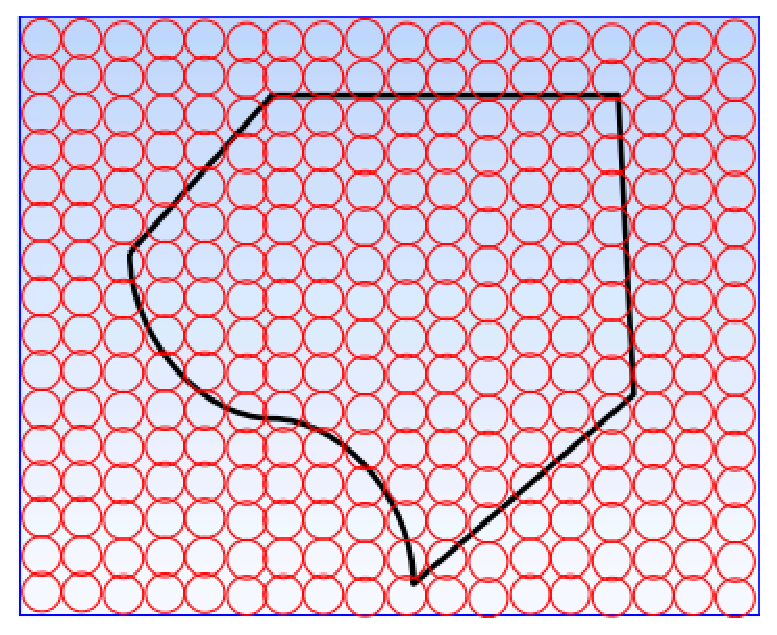
\includegraphics[width=0.95\textwidth,height=5cm]{figures/irregularity.eps}
  \caption{不规则图形面积计算}\label{fig:irr-mc}
  \end{minipage}
  \begin{minipage}[t]{0.3\linewidth}
  \centering
  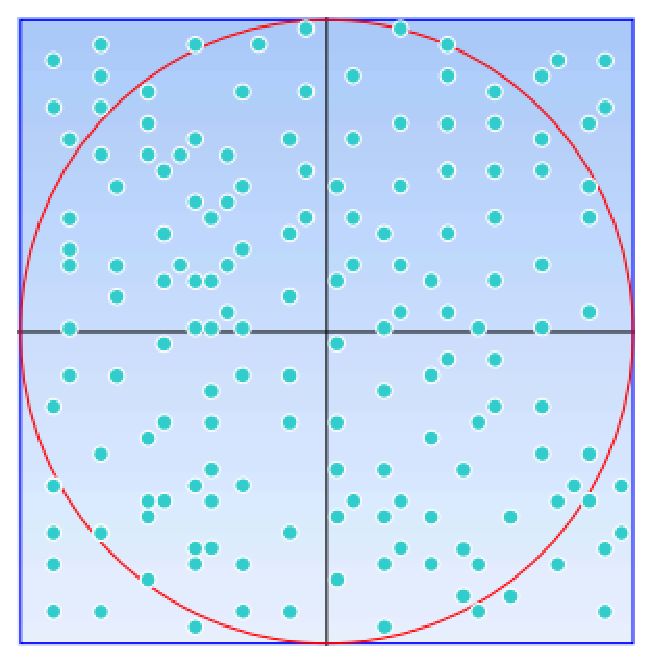
\includegraphics[width=0.95\textwidth,height=5cm]{figures/pi.eps}
  \caption{估计无理数$\pi$的值}\label{fig:pi-mc}
  \end{minipage}
  \begin{minipage}[t]{0.3\linewidth}
  \centering
  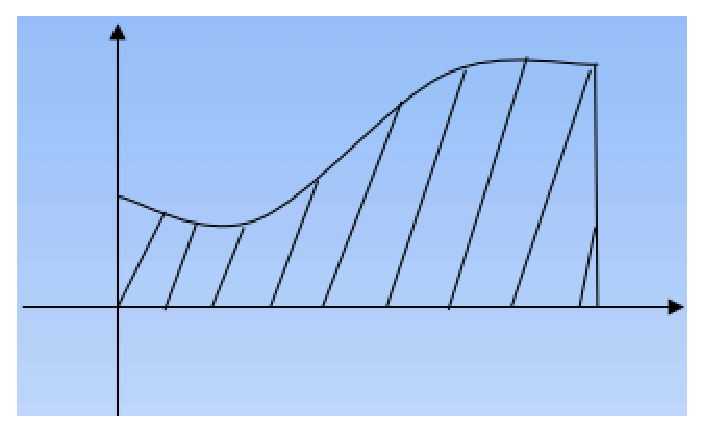
\includegraphics[width=0.95\textwidth,height=5cm]{figures/integration.eps}
  \caption{定积分计算}\label{fig:int-mc}
  \end{minipage}
\end{figure}

蒙特卡罗方法的模拟过程随机,也适合解决一些确定性问题。通常,蒙特卡罗方法包括两个基本步骤:1)利用计算机生成服从某种分布的随机样本,2)对样本做统计分析。当所求问题与某种随机事件出现的概率,或者某个随机变量的期望值存在对应关系时,我们通过“模拟实验”估计随机事件的概率,或随机变量的某些数字特征,并将其作为问题的解。由于蒙特卡罗方法需要生成大量的随机数,并且绝大多数分布都可以使用均匀分布$U(0,1)$构造,我们下面介绍几种生成服从均匀分布$U(0,1)$样本的方法。
\begin{proposition}[平方取中法]%(Middle Square Method, John von Neumann)
任取一个$m$位的整数$z_0$,依次使用$z_{i-1}^2$的中间$m$位构造序列$\{z_i\}_{i=1}^n$,则有\[x_i=z_i/10^m\sim U(0,1), i = 1, 2,\ldots,n.\]
\end{proposition}

\begin{proposition}[倍积取中法]
任取一个$m$位的整数$z_0$与$y$,依次使用$yz_{i-1}$的中间$m$位构造序列$z_i$,则有\[x_i=z_i/10^m\sim U(0,1), i = 1, 2,\ldots,n.\]
\end{proposition}

\begin{proposition}[一阶线性同余法]%(Linear Congruential Method)
指定$m=999563$、$y=47001$和初值$z_0=671800$,根据\[z_i=yz_{i-1} \pmod{m}\] 构造序列$\{z_i\}_{i=1}^n$,则有\[x_i=z_i/m\sim U(0,1), i = 1, 2,\ldots,n.\]
\end{proposition}

\begin{proposition}[一阶混合同余法]
指定$m=999563$、$w=1234$、$y=47001$ 和初值$z_0=671800$,根据\[z_i=w + yz_{i-1} \pmod{m}\] 构造序列$\{z_i\}_{i=1}^n$,则有\[x_i=z_i/m\sim U(0,1), i = 1, 2,\ldots,n.\]
\end{proposition}

\begin{proposition}[S阶混合同余法]
指定$m, w, y_1, y_2, \ldots, y_s$与$z_{-s+1}, z_{-s+2}, \ldots, z_0$,根据\[z_i=w + \sum\limits_{k=1}^s y_k z_{i-k} \pmod{m}\]构造序列$\{z_i\}_{i=1}^n$,则有\[x_i=z_i/m\sim U(0,1), i = 1, 2,\ldots,n.\]
\end{proposition}

随机数的生成方法具有重要用途,比如我们可以利用$U(0,1)$上的随机数间接地生成服从其他分布的随机数。

假设离散随机变量$X$的分布列是$P(X=x_i)=p_i, i=1,2,\ldots,n$,它的分布函数为
\begin{equation}
    F(x) = \left\{
    \begin{array}{rl}
    0, & x<x_1,\\
    p_1, & x_1\le x<x_2,\\
    p_1 + p_2, & x_2\le x<x_3,\\
    \cdots & \cdots\\
    \sum\limits_{i=1}^k p_i, & x_k \le x < x_{k+1}, \\
    \cdots & \cdots\\
    1, & x_n \le x.
    \end{array}
    \right.
\end{equation}
我们生成一个$U(0,1)$上的随机数$u$,如果$0\le u < F(x_1)$,则随机数为$x=x_1$。如果存在$F(x_{k-1})\le k < F(x_k)$,则随机数为$x=x_k$。

\begin{theorem}[反函数法]
假设随机变量$X\sim U(0,1)$,$F(z)$是一个连续分布函数且存在反函数,则随机变量$Z=F^{-1}(X)$的分布函数为$F(z)$。
\end{theorem}

\begin{property}
假设随机变量$X\sim U(0,1)$,对任意的$a,b\in \mathbb R$,只要$a<b$,则有
\[
    Z = a + (b-a)X\sim U(a,b).
\]
\end{property}
\begin{property}
假设随机变量$X\sim U(0,1)$,对任意的$\lambda,k>0$都有
\[
    Z=\big[-\frac{1}{\lambda}\ln(1-X)\big]^{1/k}
\]
服从参数为$\lambda,k$的\textbf{Weibull分布}$W(\lambda,k)$
\footnote{1927年,法国数学家Maurice Fr\'{e}chet\cite{frechet1927loi}最先给出此分布的定义。1933年Paul Rosin和Erich Rammler\cite{rossin1933laws}首次将其应用到碎末尺寸分布的研究。1951年,瑞典数学家和工程师Waloddi Weibull\cite{weibull1951statistical}对其进行详细解释。Weibull分布比\textbf{对数正态分布}具有更大的适用性,它是可靠性分析及轴承寿命检验的理论基础,被广泛应用于各种滚动轴承的寿命试验及高应力水平下的材料疲劳试验。},即
\begin{equation}
    f(x;\lambda,k) = \left\{
        \begin{array}{ll}
            \frac{k}{\lambda} (\frac{x}{\lambda})^{k-1} \exp\{-(\frac{x}{\lambda})^k\}, & x\ge 0,\\
            0,& x<0.
        \end{array}
    \right.
\end{equation}
当$k=1$时,$Z\sim \mathrm{Exp}(1/\lambda)$。
\end{property}

\begin{theorem}[Box-Muller方法]
假设$X_1\sim U(0,1), X_2\sim U(0,1)$,且$X_1,X_2$相互独立,则变量
\[
    Z_1=(-2\ln X_1)^{1/2} \cos (2\pi X_2)
\]
和变量
\[
    Z_2=(-2\ln X_1)^{1/2} \sin (2\pi X_2)
\]
相互独立,并且都服从标准正态分布$N(0,1)$。
\end{theorem}

\begin{theorem}
假设$X_1,X_2,\ldots,X_n$是$n$个独立同分布于$U(0,1)$的随机变量,则有$E(X_i)=1/2$,$\var(X_i)=1/12$。由Linderberg-Levy中心极限定理知,当$n\rightarrow \infty$时,
\begin{equation}
    Y = \frac{\sum\limits_i X_i - n/2}{\sqrt{n/12}} \sim N(0,1).
\end{equation}
当$n=12$时,$Y=\sum\limits_i X_i - 6$近似服从$N(0,1)$。
\end{theorem}
利用Box-Muller方法或者中心极限定理,我们可以在均匀分布的基础上构造出标准正态分布,进而构造出一般正态分布、三大抽样分布等,从而可以生成相应分布下的随机数。为了能够处理特别高维的概率分布随机抽样,提高随机抽样的效率问题,人们开始研究高级的随机模拟技术。

\subsection{马尔科夫链蒙特卡罗法}
1953年,Nicholas Metropolis等人\cite{metropolis1953equation} 提出一种新的随机模拟方法\textbf{马尔科夫蒙特卡罗法}(Markov Chain Monte Carlo,MCMC)(也称\textbf{动态蒙特卡罗方法}),70年代Keith Hastings\cite{hastings1970monte}将其扩展为更一般的形式,称为\textbf{Metropolis-Hastings算法}。Metropolis-Hastings 算法是MCMC的基础方法,并陆续演化出许多新的抽样方法,比如目前在MCMC 方法中最常用的\textbf{Gibbs抽样}。2009年,斯坦福大学统计学教授Persi Diaconis\cite{diaconis2009markov}使用MCMC 方法成功破解犯人密码。

1984年,Stuart Geman和Donald Geman\cite{geman1984stochastic}两兄弟提出一种新的抽样方法:Gibbs抽样,它是Metropolis-Hastings算法的一个特例($\alpha=1$),用于抽取服从多元分布的样本。

\section{参数估计}
人口普查中心要确定全国人口的身高分布,它不可能去统计全国所有人口的身高,只能做出一个模型假设,利用一定的采样数据评估模型的参数。比如,假设人口身高服从正态分布,人口普查中心只要从不同地区采样统计一部分人口的身高数据,然后通过各种统计方法估计人口正态分布的均值和方差两个参数。一般地,参数估计的形式有两种:\textbf{点估计}与\textbf{区间估计}。前者给出一个具体的数值,后者是给出未知参数的一个区间,可以反映参数估计结果的精度。我们首先介绍三种常用的点估计方法:\textbf{最大似然估计}(Maximum Likelihood Estimate,MLE)、\textbf{贝叶斯估计}(Bayesian Estimate)和\textbf{最大后验估计}(Maximum a Posteriori Estimate,MAP),再介绍区间估计的内容。

\subsection{最大似然估计}
最大似然估计最早由高斯提出,1912年Fisher再次提出,并证明了此方法的一些性质。它提供了一种给定观测数据评估模型参数的方法,即在模型确定的条件下,估计模型的参数。最大似然估计假设所有观测数据$X=\{x_1,\ldots,x_n\}$独立同分布于含参总体分布$p(x; \theta)$,并称它们的联合概率
\[
    p(X;\theta) = p(x_1,x_2,\ldots, x_n; \theta) = \prod\limits_i p(x_i; \theta)
\]
为\textbf{似然函数}。最大似然估计对参数$\theta$不作任何假设,直接从参数空间搜索一个可以使似然函数最大化的最优值,记作$\hat \theta_\mathrm{MLE}$:
\begin{equation}
   \hat \theta_\mathrm{MLE} = \argmax\limits_\theta p(X;\theta) = \argmax\limits_\theta \prod\limits_i p(x_i; \theta).
\end{equation}
由于连乘形式的似然函数不容易直接优化,通常对其应用对数变换转换为加和形式。根据对数函数的单调性可知,最大化似然函数等价于最大化对数似然函数,则有:
\begin{equation}
   \hat \theta_\mathrm{MLE} = \argmax\limits_\theta \log p(X;\theta) = \argmax\limits_\theta \sum\limits_i \log p(x_i; \theta).
\end{equation}

\begin{example}[序例\ref{eg:pistat}]
\begin{figure}[htbp]
  \centering
  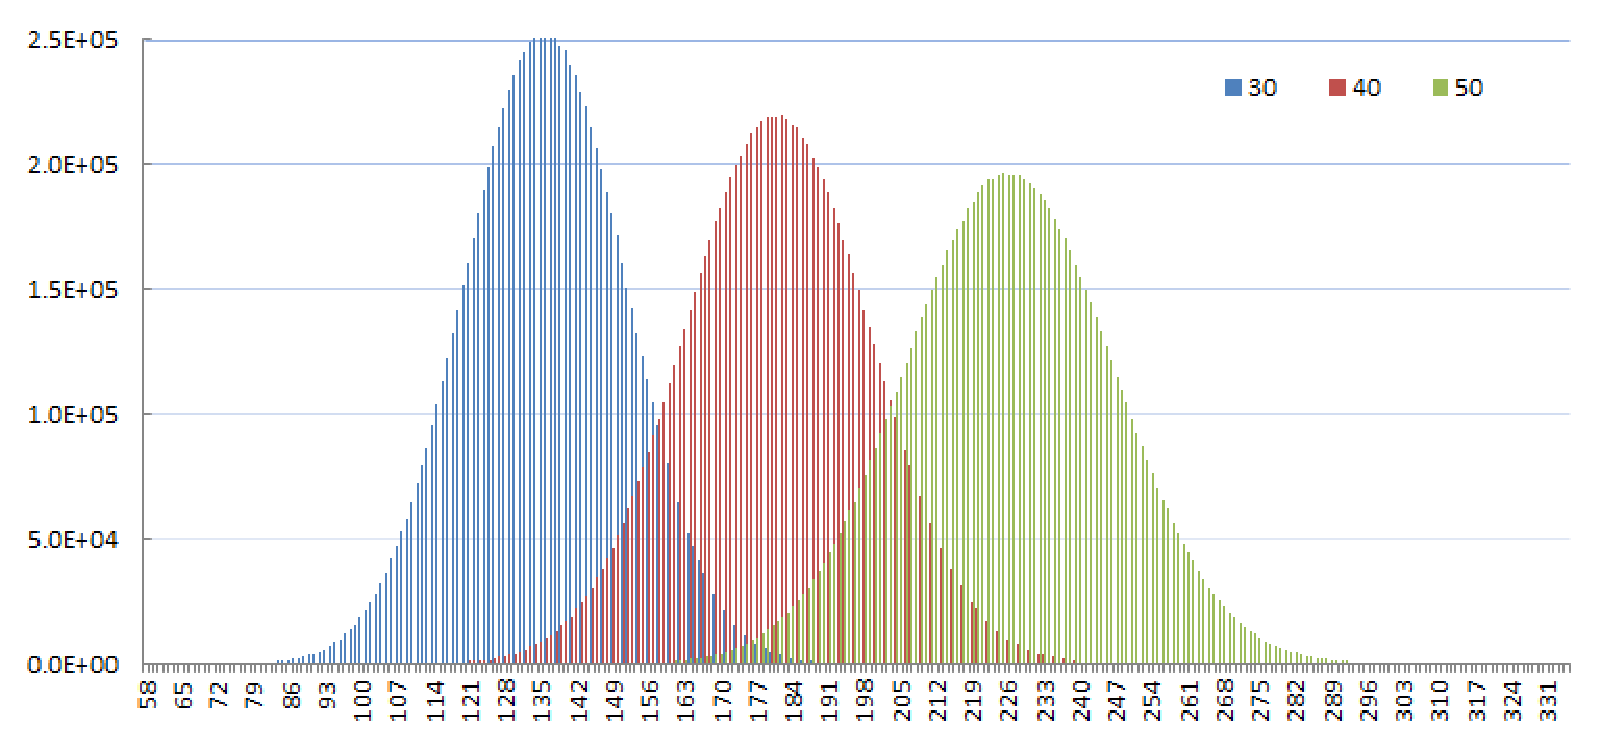
\includegraphics[width=0.85\textwidth, height=6cm]{figures/pisumdist.eps}\\
  \caption{圆周率$\pi$值前1,000万位小数连续数字串加和分布图}\label{fig:pisumdist}
\end{figure}
在观察圆周率$\pi$的单个数字的分布状况以后,我们进而考察连续数字串的特征。对小数点后的连续的数字串加和,分析不同长度数字串数字加和的分布,如图
\ref{fig:pisumdist} 所示,数字串长度从左至右分别是30、40和50,呈现出明显的正态分布特征,横轴是数字串的和,纵轴对应加和出现的频次。如果记数字串加和、频次统计数据为$\{(x_i,n_i),i\in \mathbb N\}$,我们利用这些统计数据,确定正态分布参数的最大似然估计。
假设$X\in N(\mu,\sigma)$,使用固定长度的数字串观测数据建立对数似然函数
\[
\begin{array}{lcl}
    L(x_1,x_2,\ldots; \mu,\sigma) &=& \log \prod\limits_i \big[\frac{1}{\sqrt{2\pi} \sigma} \exp\big\{-\frac{(x_i-\mu)^2}{2\sigma^2}\big\} \big]^{n_i}\\
    & = & \sum\limits_i n_i \big[\log \frac{1}{\sqrt{2\pi} \sigma} - \frac{(x_i-\mu)^2}{2\sigma^2}\big]\\
    & = & (-\log \sqrt{2\pi} - \log\sigma) \sum\limits_i n_i - \frac{1}{2\sigma^2} \sum\limits_i n_i (x_i-\mu)^2,
\end{array}
\]
从而可以确定参数$\mu$和$\sigma$的最大似然估计$\hat \mu_\mathrm{MLE}$和$\hat \sigma_\mathrm{MLE}$,则有
\[
    \hat \mu_\mathrm{MLE} = \sum\limits_i \omega_i x_i,~~~\hat \sigma_\mathrm{MLE} = \sqrt{\sum\limits_i \omega_i (x_i-\hat \mu_\mathrm{MLE})^2},~~~\omega_i = \frac{n_i}{\sum\limits_i n_i},~~~\sum\limits_i \omega_i = 1,
\]
所以$\hat \mu_\mathrm{MLE}^{30}=136$,$\hat \sigma_\mathrm{MLE}^{30}=15.72$;$\hat \mu_\mathrm{MLE}^{40}=181$,$\hat \sigma_\mathrm{MLE}^{40}=18.14$;$\hat \mu_\mathrm{MLE}^{50}=226$,$\hat \sigma_\mathrm{MLE}^{50}=20.27$。
\end{example}

\subsection{贝叶斯估计}
在统计学中有两大学派:频率学派(Frequentists,也称经典学派)与贝叶斯学派(Bayesians)。频率学派认为,统计推断是根据样本信息对总体分布或总体特征进行推断,主要使用两种信息:\textbf{总体信息}和\textbf{样本信息}。贝叶斯学派认为,在总体信息与样本信息之外,统计推断还应该使用第三种信息:\textbf{先验信息}(Prior Information)。贝叶斯统计学与经典统计学的差别就在于是否利用先验信息。贝叶斯学派的一个基本观点是:任意一个未知参数都可看作是随机变量,可以使用一个概率分布描述它,这种分布称作\textbf{先验分布}(Prior Distribution)。在获得样本信息之后,总体分布、样本与先验分布通过贝叶斯公式结合起来,构造出关于未知参数的\textbf{后验分布}(Posteriori Distribution),并在后验分布的基础之上开展统计推断。现在经典学派也已经接受这种观点\cite{Lehmann2001Theory},两派的争论焦点聚集在如何利用先验信息合理地确定先验分布。

贝叶斯学派则将未知参数$\theta$看作随机变量,而总体依赖于参数的概率函数记作$p(x|\theta)$,它表示给定随机变量$\theta$的某个取值,总体的条件概率函数。基于这种思想,样本$X=\{x_1,\ldots,x_n\}$的产生实际上经历两个基本步骤:根据模型参数的先验分布$p(\theta)$产生样本$\theta$,再从条件概率分布$p(X|\theta)$ 中产生一组样本。由此,样本$X$的联合条件概率函数表示如下:
\begin{equation}
    p(X|\theta) = p(x_1,x_2,\ldots,x_n|\theta) = \prod\limits_i p(x_i|\theta),
\end{equation}
根据贝叶斯定理,给定参数的先验分布、样本的联合条件概率分布,我们可以确定后验分布:
\begin{equation}
    p(\theta|X) = \frac{p(X|\theta)p(\theta)}{p(X)} = \frac{p(X|\theta)p(\theta)}{\int_\Theta p(X|\theta) p(\theta) d\theta}.
\end{equation}
后验分布用总体和样本信息对先验分布进行调整,集中总体、样本与先验知识中所有关于参数$\theta$的信息,它比$p(\theta)$更接近于$\theta$的实际情况。
在后验分布$p(\theta|X)$的基础上估计$\theta$,目前存在两种最常用的方法:\textbf{后验期望估计}(Posteriori Mean Estimate,PME)和\textbf{最大后验估计}
(Maximum a Posteriori Estimate,MAP),统称\textbf{贝叶斯估计}。
\begin{enumerate}
  \item \textbf{后验期望估计}:使用后验分布的均值作为$\theta$的点估计,记作$\hat \theta_\mathrm{PME}$,则有
        \begin{equation}
            \hat \theta_\mathrm{PME} = E(\theta|X) = \int_\Theta \theta p(\theta|X) d\theta.
        \end{equation}
  \item \textbf{最大后验估计}:使用后验分布的密度函数最大值点作为$\theta$的点估计,记作$\hat\theta_\mathrm{MAP}$,则有
          \begin{equation}
            \max\limits_\theta p(\theta|X) = \max\limits_\theta \frac{p(X|\theta) p(\theta)}{p(X)},
          \end{equation}
        由于$p(X)$不依赖于随机变量$\theta$,忽略分母部分可得:
        \begin{equation}
            \hat\theta_\mathrm{MAP} = \argmax\limits_\theta p(\theta) \prod\limits_i p(x_i|\theta)
            = \argmax\limits_\theta \Big[\sum\limits_i \log p(x_i|\theta) + \log p(\theta)\Big].
        \end{equation}
        对比最大似然估计和最大后验估计可以发现,最大后验估计实际上是最大似然估计的规则化模型,而其规则化项正是引入的先验概率的对数。
\end{enumerate}
贝叶斯估计与最大似然估计都是通过观测数据估计模型参数,但贝叶斯估计同时利用了未知参数的先验知识。如果先验分布可以准确描述待估参数,则贝叶斯估计比最大似然估计更加准确。此外,最大似然估计中的$p(x;\theta)$和最大后验估计及贝叶斯估计中的$p(x|\theta)$形不同而义同。最大似然估计的思想源于古典学派,将未知参数$\theta$ 看作一个普通变量,则总体依赖于参数$\theta$的概率函数记作$p(x;\theta)$,表示参数空间$\Theta$中不同的$\theta$对应不同的分布。最大后验估计和贝叶斯估计则反映贝叶斯学派的思想,将未知参数$\theta$看作随机变量,而总体依赖于参数的概率函数记作$p(x|\theta)$,它表示给定随机变量$\theta$ 的某个取值,总体的条件概率函数。

从贝叶斯公式可以看出,确定先验分布是展开贝叶斯统计推断的一个基本前提。关于先验分布的确定方法很多,目前最常用的一类先验分布是\textbf{共轭先验分布}。选择共轭先验分布从数学上可以为贝叶斯统计推断提供极大的便利,这也正是\textbf{隐含狄利克雷分布}(Latent Dirichlet Allocation, LDA)的理论基础。
\begin{definition}[共轭先验分布]
假设$\theta$是总体参数,如果对任意的样本观测值$X=\{x_1,\ldots,x_n\}$,参数$\theta$的\textbf{后验分布}$p(\theta|X)$与\textbf{先验分布}$p(\theta)$属于同一个分布族(Family),则称后验分布$p(\theta|X)$与先验分布$p(\theta)$是\textbf{共轭分布}(Conjugate Distribution),先验分布$p(\theta)$是关于似然函数$p(X|\theta)$的一个\textbf{共轭先验}(Conjugate Prior)。
\end{definition}

\begin{example}
假设事件$A$在一次试验中发生的概率是$\theta$,我们对试验进行$n$次独立观测$X=\{x_1,x_2,\ldots,x_n\}$,$x_i$表示第$i$次试验事件$A$是否发生,即
\[
    x_i = \left\{
    \begin{array}{rl}
        1, & \text{事件$A$发生},\\
        0, & \text{事件$A$未发生}.
    \end{array}
    \right.
\]
对于任意的$i\in\{1,2,\ldots,n\}$,$x_i$独立且都服从两点分布。请根据观测数据确定参数$\theta$的最大似然估计$\hat \theta_\mathrm{MLE}$、最大后验估计$\hat\theta_\mathrm{MAP}$ 与后验期望估计$\hat \theta_\mathrm{PME}$。
\end{example}
\begin{solu}
由于$p(x;\theta)=\theta^x (1-\theta)^{1-x}$,构造对数似然函数
\[
    L(x_1,x_2,\ldots,x_n;\theta) = \log\prod\limits_i p(x_i;\theta) = \sum\limits_i \big[x_i \log \theta + (1-x_i)\log(1-\theta)\big],
\]
对它求关于$\theta$的导数,可以解出参数$\theta$的最大似然估计
\begin{equation}
    \hat\theta_\mathrm{MLE} = \argmax\limits_{\theta\in (0,1)}L(x_1,x_2,\ldots,x_n;\theta) = \frac{1}{n} \sum\limits_i x_i \triangleq \frac{z}{n}.
\end{equation}
其中$z=\sum\limits_i x_i$表示$n$次试验事件$A$发生的次数。根据贝叶斯建议的“等同无知”原则假定参数$\theta$的先验分布为均匀分布$U(0,1)=\mathrm{Beta}(1,1)$,则有
\[
    p(\theta) = \frac{1}{1-0} = 1, 0<\theta<1,
\]
可以确定参数$\theta$与观测数据的联合分布为
\[
    p(X,\theta) = p(X|\theta) p(\theta) = \prod\limits_i p(x_i|\theta) = \prod\limits_i [\theta^{x_i} (1-\theta)^{1-x_i}] = \theta^z (1-\theta)^{n -z}.
\]
现在我们可以直接确定最大后验估计
\begin{equation}
    \hat\theta_\mathrm{MAP} = \argmax\limits_{\theta\in (0,1)} p(X,\theta) = \hat\theta_\mathrm{MLE} = \frac{z}{n}.
\end{equation}
根据贝叶斯定理,给定观测数据$X=\{x_1,x_2,\ldots,x_n\}$的条件下,我们可以确定参数$\theta$的后验概率
\[
    p(\theta|X) = \frac{p(X,\theta)}{\int_0^1 p(X,\theta) d\theta}, 1<\theta < 1.
\]
我们知道
\[
    \int_0^1 \theta^z (1-\theta)^{n-z} d\theta = \frac{\Gamma(z+1)\Gamma(n-z+1)}{\Gamma(z+2)},
\]
从而可得后验概率
\[
    p(\theta|X) = \frac{\Gamma(z+1)\Gamma(n-z+1)}{\Gamma(z+2)} \theta^z (1-\theta)^{n -z}, 1<\theta < 1.
\]
结果表明$\theta|X\sim \mathrm{Beta}(z+1,n-z+1)$,参数$\theta$的后验期望估计为
\begin{equation}
    \hat\theta_\mathrm{PME} = E(\theta|X) = \frac{z+1}{n+2}.
\end{equation}
\end{solu}

\subsection{区间估计}
区间估计的目标是确定两个统计量
\[
    \hat \theta_L=\hat\theta_L(x_1,\ldots,x_n) < \hat \theta_U=\hat\theta_U(x_1,\ldots,x_n),
\]
利用样本观测值,使$\theta$以概率$P(\hat\theta_L \le \theta \le \hat\theta_U)$落入区间$[\hat\theta_L,\hat\theta_U]$内。自然地,区间长度$\hat\theta_U-\hat\theta_L$越大,参数$\theta$落入区间$[\hat\theta_L,\hat\theta_U]$的可能性就越高。最理想的情景是\textbf{高概率短区间}:参数$\theta$以很高的概率落入一个狭窄的区间$[\hat\theta_L,\hat\theta_U]$。为此,我们限定参数$\theta$ 落入区间$[\hat\theta_L,\hat\theta_U]$内的概率上界,并引出\textbf{置信区间}(Confidence Interval)的概念。

\begin{definition}
假设$\theta\in \Theta$是总体的一个参数,$x_1,x_2,\ldots,x_n$是取自总体的$n$个样本,给定一个$0<\alpha<1$,如果存在两个统计量$\hat \theta_L=\hat\theta_L(x_1,\ldots,x_n)$和$\hat \theta_U=\hat\theta_U(x_1,\ldots,x_n)$,对任意的$\theta\in \Theta$,都有
\begin{equation}
    P_\theta(\hat\theta_L \le \theta \le \hat\theta_U) \ge 1-\alpha,
\end{equation}
则称随机区间$[\hat\theta_L,\hat\theta_U]$是$\theta$的\textbf{置信水平}(Confidence Level)为$1-\alpha$的\textbf{置信区间},$\hat\theta_L$和$\hat\theta_U$分别称作$\theta$的\textbf{置信下限}和\textbf{置信上限}。如果对任意的$\theta\in \Theta$,都有
\begin{equation}
    P_\theta(\hat\theta_L \le \theta \le \hat\theta_U) = 1-\alpha,
\end{equation}
则称$[\hat\theta_L,\hat\theta_U]$是$\theta$的$1-\alpha$\textbf{同等置信区间}。
\end{definition}

\section{假设检验}
\textbf{参数估计}(Parameter Estimation)和\textbf{假设检验}(Hypothesis Testing)是统计推断的主要内容,本节开始介绍假设检验的内容。我们从下面四个例子引出假设检验问题。
\begin{example}\label{eg:packingmachine}
某药品生产车间用粉剂定量自动包装机包装粉剂药品,每袋标准重量为50 mg。长期实践表明该设备包装的这一药品重量服从正态分布,且标准差为1.5 mg。现从某天的包装产品中随机抽取9袋,精确秤得它们的重量分别为
\[49.5, 50.6, 51.8, 52.1, 49.3, 51.1, 52.0, 51.5, 50.0\]
它们的平均值为50.9 mg,那么当日该包装机是否正常工作?
\end{example}
\begin{example}\label{eg:metalprod}
某工厂生产的合金强度服从正态分布$N(\theta,16)$,其中$\theta$的设计值不低于110 Pa。为保证质量,该厂每天对生产情况做例行检查,以判断生产是否正常进行。某天从生产中随机抽取25块合金,测得强度值为$x_1,\ldots,x_25$,其均值为$\bar x=108$ Pa,问当日生产是否正常?
\end{example}
\begin{example}\label{eg:alterpara}
假设总体$X\sim N(\theta,\sigma^2)$,$\sigma^2$已知,而$\theta$只能取两个值$\theta_0$或者$\theta_1$并且$\theta_0<\theta_1$,现从总体$X$中抽取的容量为$n$的样本$x_1,x_2,\ldots,x_n$,那么总体的均值是$\theta_0$还是$\theta_1$?
\end{example}
\begin{example}\label{eg:pollutedmilk}
将0.1 ml受细菌污染的牛奶均匀涂在1 cm$^2$的切片上,用显微镜观察切片每个小网格内的细菌菌落数目。根据400(20$\times$20)个小网格的计数结果,统计出如表
\ref{tbl:pollutedmilk}所示。试问菌落数是否服从泊松分布?
\begin{table}[htbp]
    \caption{污染牛奶切片菌落统计表}
    \centering
    \begin{tabular}{|l|l|l|l|l|l|l|l|l|l|l|l|l|l|l|l|l|l|l|l|l|}
      \hline
       菌落数 & 0 & 1 & 2 & 3 & 4 & 5 & 6 & 7 & 8 & 9 & 10 & 19\\
      \hline
       频~~~~数 & 56 & 104 & 80 & 62 & 42 & 27 & 9 & 9 & 5 & 3 & 2 & 1\\
      \hline
    \end{tabular}
    \label{tbl:pollutedmilk}
\end{table}
\end{example}


假设检验是一种根据简单随机抽样抽取的样本信息来判别总体是否具有某种性质的统计推断方法。两个例子代表两类假设检验问题,分别属于参数和非参数假设检验问题。\textbf{参数假设检验}在已知总体分布函数类型的前提下,对分布函数的未知参数提出某种假设,然后利用样本信息对所提假设进行检验,根据检验结果作出\textbf{接受}或者\textbf{拒绝}所提假设的判断。\textbf{非参数假设检验}是在总体分布函数类型未知的条件下,根据样本信息对分布类型的假设进行检验,从而对总体分布类型作出判断。本节重点在参数假设检验(例\ref{eg:packingmachine}、\ref{eg:metalprod}和\ref{eg:alterpara}),下一节通过例\ref{eg:pollutedmilk}具体介绍非参数假设检验。

\subsection{参数假设检验}
一般地,假设检验包含五个主要步骤:建立假设、选择检验统计量并给出拒绝域形式、选择显著性水平、给出拒绝域、作出判断。

\begin{enumerate}[Step 1.]
  \item
  \textbf{建立假设}:假设检验需要把一个被检验的假设称作\textbf{原假设}(Null Hypothesis),记作$H_0$。通常,原假设无法轻易否定。当$H_0$被拒绝时而接受的假设称作\textbf{备择假设}(Alternative Hypothesis),记作$H_1$。两个假设$H_0$和$H_1$成对出现。在例\ref{eg:packingmachine}中,包装机包装药品的重量服从正态分布$N(\theta,\sigma^2)$,我们已知参数$\sigma=1.5$,对于判断机器包装重量的均值是否等于$\theta_0=50$ mg,可以建立如下两个假设:\[H_0: \theta\in \Theta_0 =\{\theta: \theta = \theta_0\} ~~~~~~ \textrm{vs}  ~~~~~~ H_1: \theta\in \Theta_1 =\{\theta: \theta \ne \theta_0\}.\]
  这种形式的参数假设检验称作\textbf{双侧检验}(Two-sided Testing),还有一种形式的假设检验称作\textbf{单侧检验}(One-sided Testing):
  \[H_0: \theta\in \Theta_0 =\{\theta: \theta \ge \theta_0\} ~~~~~~ \textrm{vs}  ~~~~~~ H_1: \theta\in \Theta_1 =\{\theta: \theta < \theta_0\},\] 或者\[H_0: \theta\in \Theta_0 =\{\theta: \theta \le \theta_0\} ~~~~~~ \textrm{vs}  ~~~~~~ H_1: \theta\in \Theta_1 =\{\theta: \theta > \theta_0\}.\]
  \item
  \textbf{选择检验统计量,给出拒绝域形式}:根据样本数据对原假设进行判断总是通过一个统计量来完成,这个统计量称作\textbf{检验统计量}。通常,检验统计量$T(x_1,x_2,\ldots,x_n)$也是一个\textbf{充分统计量}。在确定检验统计量以后,从而可以建立原假设被拒绝的\textbf{拒绝域}(Rejection Region),它是样本空间的一个子集,记作$W$。一般地,拒绝域的形式依赖于参数假设检验的形式,如果是单侧检验,则拒绝域是一个连续的样本空间子集:
  \[W=\{(x_1,x_2,\ldots,x_n): T(x_1,x_2,\ldots,x_n; \theta) \le \tau\}\]或者\[W=\{(x_1,x_2,\ldots,x_n): T(x_1,x_2,\ldots,x_n; \theta) \ge \tau\}.\]
  如果是双侧检验,则拒绝域由两个不相交的连续样本空间子集构成:
  \[W=\{(x_1,x_2,\ldots,x_n): |T(x_1,x_2,\ldots,x_n; \theta)| \ge \tau\}.\]
  当拒绝域确定后,检验的判断准则也相应地确定。如果$(x_1,x_2,\ldots,x_n)\in W$,则认为$H_0$不成立,拒绝原假设;如果$(x_1,x_2,\ldots,x_n)\in A$,则认为$H_0$成立,接受原假设,$A$称作\textbf{接受域}(Acceptance Region)。
  例\ref{eg:packingmachine}所示的假设检验属于双侧检验,由于$\bar x\sim N(\mu, \sigma^2/n)$,我们选择统计量
  \[T(x_1,x_2,\ldots,x_n; \theta)=\frac{\bar x - \mu_0}{\sigma/\sqrt{n}},\]并构造双侧拒绝域。
  \item
  \textbf{选择显著性水平}:由于抽样的随机性和小概率事件的发生,假设检验可能犯下两类错误。第一类错误(Type I Error)是$H_0$为真,但是样本观测值落在拒绝域内,从而拒绝原假设$H_0$,其发生的概率称作\textbf{拒真概率},记作$\alpha$,即
  \[\alpha = P(\text{拒绝}H_0|H_0\text{为真}).\]%=P((x_1,x_2,\ldots,x_n)\in W)
  第二类错误(Type II Error)是$H_1$为真,但是样本观测值落在接受域内,从而接受原假设$H_0$,其发生的概率称作\textbf{纳伪概率},记作$\beta$,即
  \[\beta = P(\text{接受}H_0|H_1\text{为真}).\]%=P((x_1,x_2,\ldots,x_n)\in \overline W)
  一般地,拒真概率越小,则纳伪概率越大;反之,拒真概率越大,纳伪就概率越小。为了平衡两种错误,统计学家Jerzy Neyman与Egon Pearson提出显著性检验优先的基本原则:在控制出现第一类错误$\alpha$的条件下,寻求使出现第二类错误$\beta$尽可能小的检验。$\alpha$也称\textbf{显著性水平}(Significance Level),通常取值$\{0.01,0.05,0.10\}$,$1-\alpha$称作\textbf{置信水平}(Confidence Level),$1-\beta$称作\textbf{检验效能}(Power of Testing)。
  \item \textbf{给出拒绝域}:
  在确定显著性水平后,我们可以确定出检验的拒绝域$W$。对于例\ref{eg:packingmachine},如果取$\alpha=0.05$,则拒绝域
  \[
    W=\{(x_1,x_2,\ldots,x_n): |\frac{\bar x-\theta_0}{\sigma\sqrt n}| \ge \Phi^{-1}(\alpha/2)\} = \{(x_1,x_2,\ldots,x_n): |\frac{\bar x-\theta_0}{\sigma/\sqrt n}| \ge 1.96\}.
  \]
  \item \textbf{作出判断}:
  由于$\bar x=50.9$,则\[
    \frac{\bar x - \theta_0}{\sigma/\sqrt n}=\frac{50.9-50}{1.5/3}=1.8 < 1.96
  \]
  接受原假设$H_0$。
\end{enumerate}

\subsection{非参数假设检验}%Nonparametric Hypothesis Test
\begin{definition}[经验分布函数]
设$X_1, X_2, \ldots, X_n$是来自总体$X$的样本,$x_1, x_2, \ldots, x_n$是对应观察值,将它们按照观察值的大小递增顺序排列生成$x_{(1)}\le x_{(2)}\le \cdots \le x_{(n)}$,构造函数:
\[
    F_n(x) = \left\{
    \begin{array}{rl}
    0, & x<x_{(1)},\\
    \dfrac{k}{n}, & x_{(k)}\le x<x_{(k+1)}, k = 2,3,\ldots, n-1,\\
    1, & x \ge x_{(n)}.
    \end{array}
    \right.
\]
则称$F_n(x)$是总体$X$的\textbf{经验分布函数}(Empirical Distribution Function)。对应地,总体$X$的分布函数$F(x)$称作\textbf{理论分布函数}(Theoretical Distribution Function)。
\end{definition}

在20世纪30年代,前苏联统计学家Valery Ivanovich Glivenko与意大利数学家Francesco Paolo Cantelli证明了一个极限定理,并成为统计学基础理论一个重要的结论。
\begin{theorem}[Glivenko-Cantelli定理]
设$x_1,x_2,\ldots, x_n$是取自总体分布函数为$F(x)$的样本,$F_n(x)$是其经验分布函数,当$n\rightarrow +\infty$时,有
\[
    P\{\sup\limits_{-\infty<x<+\infty} |F_n(x) - F(x)| \rightarrow 0\} = 1.
\]
\end{theorem}
Glivenko-Cantelli定理表明,当$n$充分大时,经验分布函数是总体分布函数$F(x)$的一个良好的近似。经典统计学中一切统计推断都以样本为依据,其理由就在于此。
我们可以利用Glivenko-Cantelli定理进行非参数假设检验:设总体$X$的分布函数为$F(x)$,对一个给定的分布$F_0(x)$,考虑原假设$H_0: F(x) = F_0(x)$,
根据Glivenko-Cantelli定理:当样本容量$n$充分大时,样本的经验分布函数$F_n(x)$是总体$X$分布函数$F(x)$的一个很好的近似。当原假设$H_0$为真时,$F_n(x)$与$F_0(x)$之间的差应该是一个小量。

\begin{theorem}
设总体$X$的分布函数$F(x)$连续,$X_1,X_2,\ldots, X_n$是来自总体$X$的样本,则对任意的分布函数$F_0(x)$,如果$H_0:F(x)=F_0(x)$成立,必然有
\begin{equation}
    \lim\limits_{n\rightarrow +\infty} P(D^{(n)} < \frac{\lambda}{\sqrt n}) = K(\lambda),
\end{equation}
其中,$D^{(n)}$称作\textbf{Kolmogorov统计量}
\begin{equation}
    D^{(n)} = \sup\limits_{-\infty<x<+\infty} |F_n(x) - F_0(x)| = \max\limits_{1\le i\le n} \big\{|\frac{i}{n} - F_0(x_{(i)}|,|\frac{i-1}{n} - F_0(x_{(i)}|\big\}
\end{equation}
是经验分布函数$F_n(x)$与$F_0(x)$的最大间隔,满足\textbf{分布无关性}。$K(\lambda)$是Kolmogorov分布密度函数
\begin{equation}
    K(\lambda) =\left\{
    \begin{array}{rl}
    \sum\limits_{k=-\infty}^{+\infty} (-1)^k e^{-2k^2\lambda^2}, & \lambda > 0,\\
    0, & \lambda \le 0.
    \end{array}
    \right.
\end{equation}
\end{theorem}

\begin{definition}[Kolmogorov–Simrnov检验]
设总体$X$的分布函数$F(x)$连续,$X_1,X_2,\ldots, X_n$是来自总体$X$的样本,则对任意的分布函数$F_0(x)$,考虑原假设$H_0:F(x)=F_0(x)$,在显著性水平$\alpha$下的拒绝域形式为:
\[
    W = \{(x_1,x_2,\ldots, x_n): D^{(n)} \ge D_{1-\alpha}^{(n)}\}.
\]
其中$P(D^{(n)} \ge D_{1-\alpha}^{(n)}) = \alpha$,并且$D_{0.99}^{(n)} \approx 1.63/\sqrt n$,$D_{0.95}^{(n)} \approx 1.36/\sqrt n$,$D_{0.9}^{(n)} \approx 1.23/\sqrt n$。
\end{definition}

\subsection{显著性检验}
为了衡量模型之间是否存在显著性的差异,有两种办法:其一,直接比较数值差异,其二是确定这种差异是否具有统计显著性(Statistical Significance)。通常,数值差异并不意味着具有统计显著性差异,比如\cite{gomes2013learning}通过在多个数据集上分析基准排序学习算法发现,排序学习模型尽管相比最佳特征具有显著的数值差异,经过统计分析,这种差异不具有统计学意义。

假设存在两个系统A和B,在每个系统上都执行$n$次试验,相应的分别得到两组试验结果$X = (x_1,\ldots, x_n), Y = (y_1,\ldots, y_n)$。 由此,可以计算系统A 和B 实验结果的偏差$Z = X - Y$。$Z$包含了$n$ 次试验偏差,相应的可以利用均值($\mu$)、方差($\sigma$)、给定的置信度(如95\%),通过查询$t$分布分位数表,就可以构建偏差的置信区间(Confidence Interval)$\mu \pm t \sqrt{\sigma/n}$。如果置信区间含有0,则表明两个系统试验结果是没有显著性差异的\cite{jain1991art}。

统计显著性从统计意义上保证了系统之间实验结果的差异性是真实可信的,而非仅仅出于偶然。比如,某种疾病的治疗方案有两种:A 和B,如果通过A、B治疗方案的病人都是100位,痊愈的比例分别是100\%、50\%,显然A 方案相比B治疗效果更为显著。假设接受A方案的病人只有1个,而接受B方案的有两个,同样的治愈率(100\% 与50\%)所反映的显著性就大打折扣。再设想,如果通过相同的治疗分组,治愈率分别是66\%,60\%,那么二者的差异性就不是那么明显了
\footnote{Cancer Guide:\href{http://cancerguide.org/significance.html}{http://cancerguide.org/significance.html}}。

统计显著性具有两个基本的特点:(1)如果数值差异越大,则出于偶然性的可能性越低;(2)根据大数定理,实验的样本越大,则观察到的差异性越能够反映真实的差异。

统计检验首先假设比对组实验结果是相同的,然而从数学上估计比对组之间差异出于偶然的概率,我们称之为p 值(p-Value),p值越大,则差异显著性就越弱,反之,比如$p<0.05$,则表明差异是显著的。

给定两组样本$x = (x_1,\ldots,x_n), y = (y_1,\ldots, y_n)$,为了比较二者之间的差异,一般会选择比较两组样本的样本均值,实际上样本均值的差异并不能反映整体差异。

显著性差异是一种有量度的或然性评价。比如说$x,y$两组样本在$p=0.05$水平上具有显著性差异,也即是说两组样本具有显著性差异的可能性是95\%,另外5\%的可能性是没有差异。这5\%的差异是由随机误差造成的。

\textbf{显著性检验}(Significance Test),又称\textbf{假设检验}(Hypothesis Test),有多种检验方法,如$t$检验、$F$检验和$\chi$检验等。

$t$检验基本步骤:
\begin{enumerate}
  \item 计算样本差异
  \[
    z = (z_1,\ldots,z_n)
  \]
  其中,$z_i = y_i - x_i,i=1,\ldots,n$。
  \item 计算样本平均差异
  \[
    \bar{z} = \sum\limits_i z_i
  \]
  \item 计算样本标准差
  \[
    s_z = \sqrt{\frac{1}{n-1}\sum\limits_i (z_i - \bar{z})^2}
  \]
  \item 计算统计量$t$
  \[
    t = \frac{\bar{z}}{s_z/\sqrt{n}}
  \]
  \item 根据样本大小$n$和$p$值(通常取$p=0.05,p=0.01$),查$t$分布表:$t_p(n-1)$
  \item 如果$|t|>t_p(n-1)$,则可以断定差异显著。
\end{enumerate}

\section{Wilcoxon-Mann-Whitney检验}
Wilcoxon-Mann-Whitney检验~\cite{wilcoxon1945individual,mann1947test},是一种无参检验方法,也称Mann-Whitney U检验、Wilcoxon秩和检验(Rank Sum Test),用于检验(推断)两组随机样本(分布)之间的差异性。WMW 检验的零假设(Null Hypothesis)是两组样本取自于性质相同的分布,它不是计算平均值的差异性,而是根据两组样本名次之和,计算出U-统计量以作检验。

给定随机变量$X$的样本数据$\{x_i\}_{i=1}^m$,随机变量$Y$的样本数据$\{y_j\}_{j=1}^n$,则U-统计量定义为:
\begin{equation}
    U = \frac{1}{mn} \sum\limits_{i=1}^m \sum\limits_{j=1}^n I(x_i > y_j)
\end{equation}
U-统计量实际上是对同序概率(Concordance Probability)$P(X>Y)$的一个估计量,如果以$X$,$Y$为坐标轴绘制ROC曲线,AUC与U-统计量等价
\cite{hanely1982meaning}。

在二元分类问题中,假设$x_1,\ldots,x_m$是分类器对正例的预测结果,$y_1,\ldots,y_n$是对负例的预测结果。将所有预测结果升序排列,我们可以根据所有正例的排名计算统计量$U$:
\begin{equation}
    U = \frac{1}{mn} \big[\sum\limits_{i=1}^m r_i - \frac{1}{2} m(m-1) \big]
\end{equation}
其中,$r_i$表示预测结果$x_i$的排名。在最理想的条件下,所有正例都应该得到大于负例的预测结果,从而有
\begin{equation}
    U = \frac{1}{mn}\big[(n+1) + (n+2) + \ldots + (n+m) - \frac{1}{2} m(m-1)\big] = 1,
\end{equation}
最不济的分类器完全预测错误,对应地有
\begin{equation}
    U = \frac{1}{mn}\big[(1 + 2 + \ldots + m)  - \frac{1}{2} m(m-1)\big] = 0.
\end{equation}
综上可知,U-统计量的取值范围在$[0,1]$之间。

\section{一般加法模型}%Generalized Additive Model: GAM
\section{Copula函数}
Copula函数是一种多元分布函数,函数变量都服从均匀分布。Copula是一类重要的统计分析方法,在分析随机变量之间的相关关系时,将随机变量的概率分布从相关性结构(Dependency Structure)中独立出来,为构建非线性多元统计模型提供了一个便利的工具,可应用于金融风险管理、机器学习\cite{poczos2012copula}等领域。

1959年,Abe Sklar\cite{sklar1959fonctions}首次引入Copula,将一个$n$维概率分布函数$F$分解成\textbf{边际概率分布$F_i,i=1,\ldots,n$}与\textbf{描述分布函数中相依关系的Copula~$C$}两个部分。1981年,Berthold Schweizer与Edward Wolff\cite{schweizer1981nonparametric}最早将Copula与变量之间的相关性分析联系起来,他们在概率测度背景下的分析奠定了Copula 模型理论基础。
\begin{definition}[Copula]
假设随机向量$X=(X_1,\ldots,X_n)$的分布函数为$F$,边际概率分布为$F_i,X_i\sim F_i,i=1,\ldots,n$,分布函数$C$的变量是$[0,1]$ 上的均匀分布函数,如果
\begin{equation}
    F = C(F_1,\ldots,F_n)
\end{equation}
则称函数$C$是向量$X$的Copula。
\end{definition}

如果分布函数$F$的边际分布$F_i$是连续的,则$F_i(X_i)\sim U(0,1)$,则我们可以定义$C$为随机向量$(F_1(X_1), \ldots, F_n(X_n))$的分布函数,则有
\begin{equation}
    \begin{array}{lll}
      C(u_1,\ldots,u_n) & = & P(F_1(X_1)\le u_1, \ldots, F_n(X_n)\le u_n)) \\
       & = & P(X_1\le F_1^{-1}(u_1), \ldots, X_n\le F_n^{-1}(u_n)) \\
       & = & F(F_1^{-1}(u_1),\ldots, F_n^{-1}(u_n))
    \end{array}
\end{equation}
其中,$F_i^{-1}$表示边际函数$F_i$的广义反函数,又称“分位变换”(Quantile Transform),定义形式如下
\begin{equation}
    F_i^{-1}(t) = \inf\limits_{x}~\{x\in \mathbb R|F_i(x)\ge t, 0 < t < 1\}
\end{equation}

由于联合分布
\begin{equation}
    \begin{array}{lll}
      F(x_1,\ldots,x_n) & = & P(X_1\le x_1, \ldots, X_n\le x_n) \\
       & = & P(F_1(X_1) \le F_1(x_1), \ldots, F_n(X_n) \le F_n(x_n)) \\
       & = & C(F_1(x_1),\ldots, F_n(x_n))
    \end{array}
\end{equation}
根据定义可知,函数$C$是向量$X$的Copula。

\begin{definition}[高斯Copula函数]
假设$\Phi_R(X_1,\ldots,X_n)$是$n$元标准正态分布函数,相关系数矩阵是$R\in\mathbb R^{n\times n}$,由此可以构造出高斯Copula函数
\begin{equation}
    C_R(u_1,\ldots,u_n) = \Phi_R(\Phi_1^{-1}(u_1),\ldots,\Phi_n^{-1}(u_n))
\end{equation}
其中,$\Phi_i^{-1}(u_1)$表示标准正态分布函数的反函数。
\end{definition}

\begin{theorem}[Sklar定理]
假设$F\in \mathcal{F}(F_1,\ldots,F_n)$是边际函数为$F_i,i=1,\ldots,n$的$n$元分布函数,则存在一个边际分布是均匀分布函数的Copula函数$C\in \mathcal{F}(U_1,\ldots,U_n)$,使得
\begin{equation}
    F(x_1,\ldots,x_n) = C(F_1(x_1),\ldots,F_n(x_n))
\end{equation}
并且当$F_i,i=1,\ldots,n$连续时,则满足上面等式的Copula函数是唯一的。
\end{theorem}
给定一个Copula函数$C$,边际函数$F_i,i=1,\ldots,n$,则$C(F_1(X_1),\ldots,F_n(X_n))$定义了一个$n$元分布函数,其边际函数正是$F_i,i=1,\ldots,n$。Sklar定理
\cite{sklar1959fonctions}为Copula的应用提供了重要的理论依据。

在实际应用中,我们可以使用Copula方法从多元统计数据中构造出多元随机变量的联合分布。假设数据集中有$m$个$n$维观测数据$(X_1^i, \ldots, X_n^i),i=1,\ldots,m$ 是从联合分布$F(X_1,\ldots,X_n)$采样取得,边际分布$F_1,\ldots,F_n$都连续,则相应的真实Copula分布函数的观测数据就是
\begin{equation}
    (U_1^k,\ldots, U_n^k) = (F_1(X_1^k),\ldots,F_n(X_n^k)),~~k=1,\ldots,m
\end{equation}
事实上,真实的边际函数$F_i,i=1,\ldots,n$通常是未知的,我们可以使用经验分布函数
\begin{equation}
    \tilde F_i (x) = \frac{1}{m} \sum\limits_{k=1}^m I(X_i^k \le x), ~~i=1,\ldots,n
\end{equation}
构造出伪Copula分布观测数据
\begin{equation}
    (\tilde U_1^k,\ldots, \tilde U_n^k) = (\tilde F_1(X_1^k),\ldots,\tilde F_n(X_n^k)),~~k=1,\ldots,m
\end{equation}
由此可定义经验Copula函数
\begin{equation}
    \tilde C(u_1,\ldots,u_n) = \frac{1}{m} \sum\limits_{k=1}^m I(\tilde U_1^k \le u_1,\ldots, \tilde U_n^k \le u_n)
\end{equation}

\begin{theorem}[Fr\'{e}chet–Hoeffding定理]
对于任意的Copula函数$C:[0,1]^n\mapsto [0,1]$,任意的向量$(u_1,\ldots,u_n)\in [0,1]^n$,都满足不等式
\begin{equation}
    \max\big\{1-n+\sum\limits_i u_i,~0\big\} \le C(u_1,\ldots,u_n) \le \min\big\{u_1,\ldots,u_n\big\}.
\end{equation}
\end{theorem}
